\documentclass[a4paper,10pt, oneside, titlepage]{article}

\usepackage[spanish,es-tabla]{babel}
\usepackage[hidelinks]{hyperref}
\usepackage[utf8]{inputenc}
\usepackage[T1]{fontenc}
\usepackage{subcaption}
\usepackage{graphicx}
\usepackage{listings}
\usepackage{sectsty}
\usepackage{xcolor}

\title{Manual de Instalación de Servicios OBD-2 y Accuweather para el Agente de Respuesta SIGOAVE}
\author{Arroyo Auz Christian Xavier}
\date{}

\begin{document}
	\maketitle
	\section{Introducción}\label{Etiqueta_Introduccion}
	El agente de respuesta forma parte de un conjunto de sistemas autónomos para la gestión de accidentabilidad vehicular, este es una aplicación móvil que presenta el índice de accidentabilidad del vehículo y ciertos parámetros claves del conductor, vehículo, condiciones climatológicas y del flujo de tráfico. Adicionalmente, este agente se encarga de solicitar información procesada al servicio de siniestrabilidad vehicular (SIGOAVE). \\\newline
	\indent Además, la aplicación genera notificaciones y alertas en base a la información provista por SIGOAVE. Una de las principales características de esta aplicación móvil es que funcione de manera autónoma, pero pueda trabajar en sinergia con la aplicación móvil del agente de adquisición. \\\newline
	\indent La Figura \ref{Funcionalidad} presenta el esquema de este conjunto de sistemas autónomos.
	\begin{figure}[!h]
		\centering
		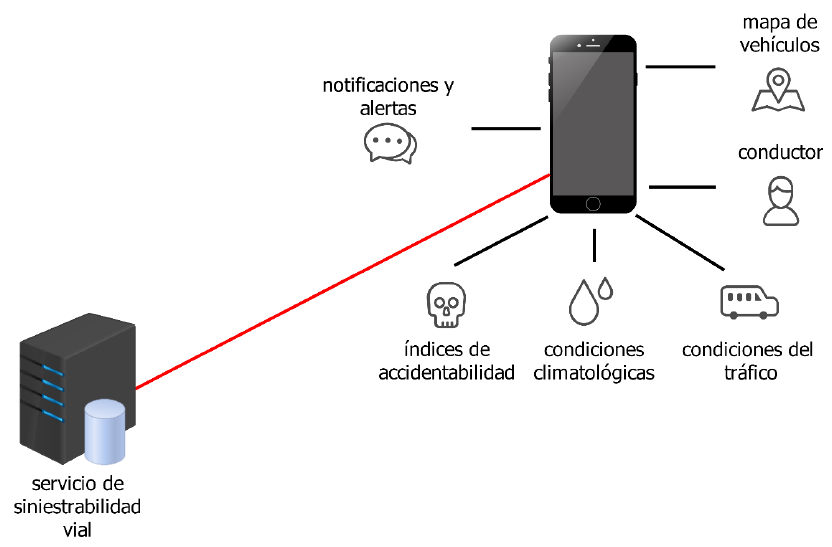
\includegraphics[width = 1\linewidth, height = 6.6cm]{Funcionalidad.png}
		\caption{Funcionalidades del Agente de Respuesta.}
		\label{Funcionalidad}
	\end{figure}
	
	\section{Objetivo}\label{Etiqueta_Objetivo}
	El objetivo principal de utilizar un OBD-II (On-Board Diagnostics) y de integrarlo en una aplicación de Android es obtener datos en tiempo real sobre el rendimiento y la salud de un vehículo. El OBD-II es un sistema de diagnóstico a bordo que está presente en la mayoría de los vehículos fabricados después de 1996. Proporciona acceso a una amplia gama de información, como códigos de diagnóstico de problemas (DTC), velocidad del motor, temperatura del refrigerante, velocidad del vehículo, entre otros. Al integrar un OBD-II con una aplicación de Android, se pueden realizar varias funciones útiles, que pueden incluir \cite{GeoTab}:
	\begin{itemize}
		\item Monitoreo en tiempo real: Obtener información en tiempo real sobre diferentes aspectos del vehículo, como la velocidad del motor, la temperatura del refrigerante, la velocidad del vehículo, etc.
		\item Diagnóstico de problemas: Leer y borrar códigos de diagnóstico de problemas (DTC), lo que permite a los usuarios identificar y solucionar problemas mecánicos o de rendimiento del vehículo.
		\item Mejora del rendimiento: Utilizar los datos proporcionados por el OBD-II para mejorar el rendimiento del vehículo, monitoreando el consumo de combustible, la eficiencia del motor, entre otros.
		\item Registro de viajes: Registrar datos de viajes, como la distancia recorrida, el tiempo de conducción, la eficiencia del combustible, etc., que pueden ser útiles para llevar un registro de los hábitos de conducción y los gastos de mantenimiento del vehículo.
		\item Seguridad: Alertar al usuario sobre condiciones peligrosas del vehículo, como el sobrecalentamiento del motor o la baja presión de aceite, para garantizar una conducción segura.
	\end{itemize}
	\indent El objetivo de utilizar AccuWeather es acceder a información meteorológica precisa y detallada para una variedad de propósitos, tanto personales como profesionales. AccuWeather es una de las principales aplicaciones y servicios de pronóstico del tiempo disponibles en la actualidad, y ofrece una amplia gama de características y datos para ayudar a los usuarios a planificar y prepararse según las condiciones meteorológicas. Algunos de los objetivos de utilizar AccuWeather incluyen \cite{AccuWeather}:
	\begin{itemize}
		\item Pronósticos precisos: AccuWeather utiliza tecnología avanzada y datos de alta calidad para proporcionar pronósticos meteorológicos precisos a corto y largo plazo. Esto ayuda a los usuarios a planificar actividades al aire libre, viajes y eventos con mayor confianza.
		\item Alertas meteorológicas: La aplicación envía alertas meteorológicas en tiempo real para condiciones peligrosas o adversas, como tormentas severas, tornados, inundaciones, nevadas intensas, entre otros. Estas alertas ayudan a mantener a los usuarios informados y seguros ante eventos climáticos extremos.
		\item Información detallada: AccuWeather ofrece información detallada sobre diversas condiciones meteorológicas, incluyendo temperatura actual, sensación térmica, velocidad y dirección del viento, humedad, índice UV, visibilidad, entre otros. Esta información es útil para tomar decisiones informadas sobre cómo vestirse, planificar actividades al aire libre y más.
		\item Mapas meteorológicos interactivos: La aplicación ofrece mapas meteorológicos interactivos que permiten a los usuarios visualizar patrones climáticos, como precipitación, nubes, temperatura y más, en tiempo real. Estos mapas ayudan a comprender mejor las condiciones meteorológicas locales y regionales.
		\item Personalización: AccuWeather permite a los usuarios personalizar la experiencia según sus preferencias, como la ubicación favorita, las unidades de medida, los tipos de alertas a recibir, entre otros. Esto garantiza que la información meteorológica sea relevante y útil para cada usuario individual.
	\end{itemize}
	\subsection{Objetivos Específicos}\label{Etiqueta_Objetivos_Especificos}
	\begin{itemize}
		\item Proporciona a los usuarios una manera conveniente de monitorear y diagnosticar el rendimiento de sus vehículos, así como de mejorar su eficiencia y seguridad.
		\item Proporcionar a los usuarios acceso a pronósticos meteorológicos precisos, alertas en tiempo real y una amplia gama de información climática detallada para ayudarles a tomar decisiones informadas y mantenerse seguros en diversas condiciones climáticas.
	\end{itemize}
	
	\section{Esquema del Modelo de Agente OBD-2}\label{Etiqueta_Modelo_Agente_OBD-2}
	Se diseñó e implementó una aplicación móvil para Android basada en el lenguaje de programación Java. La aplicación interactúa con un escáner OBD2 y un receptor GPS para recoger parámetros y la ubicación del vehículo, y con un reloj inteligente para obtener el ritmo cardíaco del conductor. Una vez que la información es generada, se realiza la obtención de los parámetros de condiciones climáticas desde un servicio climatológico y el número de accidentes de tránsito dados cerca de una ubicación especifica desde una base de datos. En primera instancia, el agente de adquisición fue usado para generar el conjunto de datos de conducción denominada POLIDriving. Esta versión del conjunto de datos incluye información del conductor, del vehículo, condiciones climáticas y accidentes de tránsito. Una vez que el conjunto de datos fue generado, el agente de adquisición tiene la funcionalidad de recoger los parámetros y almacenarlos localmente. \\\newline
	\indent El agente de respuesta usará esta información para enviar al modelo y realizar predicciones. La Figura \ref{Esquema} presenta el esquema de funcionamiento del agente de adquisición.
	\begin{figure}[!h]
		\centering
		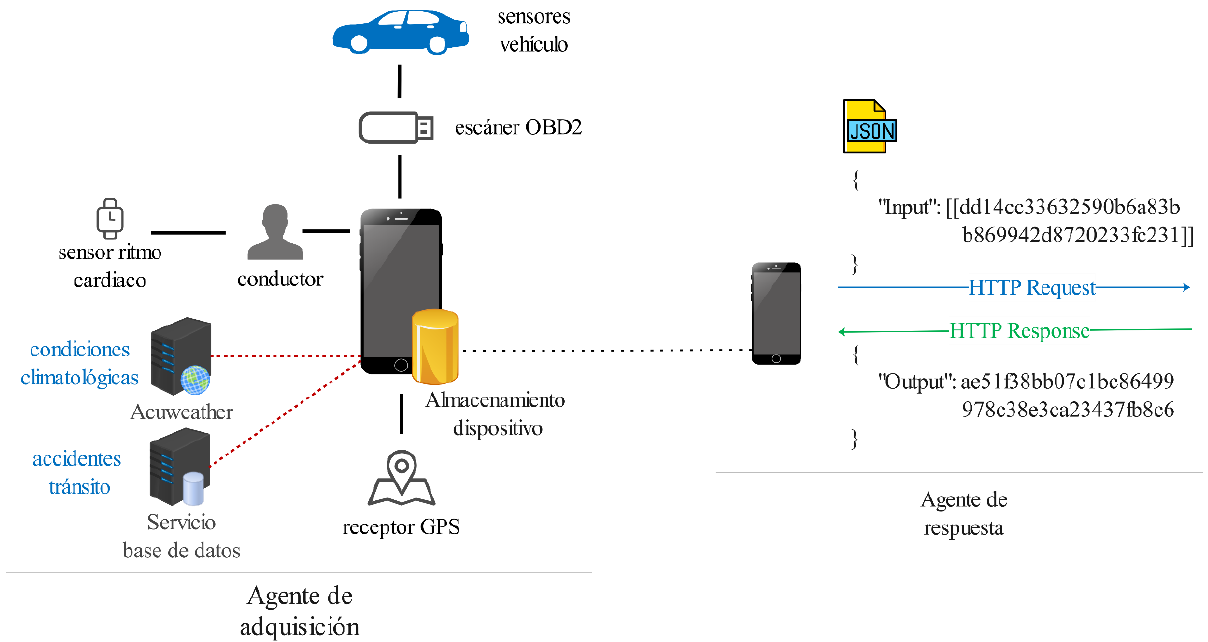
\includegraphics[width = 1\linewidth, height = 7.2cm]{Esquema.png}
		\caption{Esquema de Funcionamiento del Agente de Adquisición.}
		\label{Esquema}
	\end{figure} \\
	\indent El artículo \cite{marcillo2022systematic} y publicado en Applied Sciences (Q2), proporcionó información relacionada a fuentes de datos y atributos usados por los modelos de predicción, y a plataformas, servicios de Internet y simuladores usados para recolectar información. Esta información permitió diseñar e implementar un agente de adquisición que se ajuste a ciertos requerimientos funcionales y no funcionales. En el siguiente enlace se encuentra el conjunto de datos POLIDriving:
	\begin{itemize}
		\item \textcolor{blue}{\url{https://github.com/laboratorioAI/PIS_20_02_AGENTES_IA/tree/main/Actualizacion_2024/Dataset}}
	\end{itemize}
	
	\section{On Board Diagnostics - OBD}\label{Etiquet_OBD}
	El denominado OBD es un sistema de diagnóstico vehicular incorporado al vehículo y que tiene la función de controlar y monitorear tanto al motor como algunos otros dispositivos; dentro de estos, se puede controlar el nivel de emisiones que genera la unidad y determinar si contamina \cite{CONUEE}. \\\newline
	\indent En 1988, para reducir la contaminación en el aire, la California Air Resources Board, de Estados Unidos, determina que todos los automóviles a gasolina deben contar con el sistema OBD, que con base en dispositivos electrónicos controlará los límites de emisiones de gas. \\\newline
	\indent En el año 1996, debido a nuevas medidas contra la contaminación, se llevó a cabo la adopción del OBDII. A la fecha, se habla de que se está ajustando una norma más estricta en los contaminantes, con lo que se creará la OBDIII. \\\newline
	\indent En Europa, según la Directiva 98/69EG, los automóviles a gasolina del año 2000 en adelante, los de diésel a partir de 2003, y los camiones desde 2005 tienen que estar provistos de un OBD. \\\newline
	\indent La interfaz estándar del OBD-II no solamente es utilizada por el fabricante para sus funciones avanzadas de diagnóstico, sino también por aquellos que van más allá de lo que la ley exige. \\\newline
	\indent La siguiente etapa planeada es el OBDIII, en el que los propios automóviles se comunican con las autoridades, si se produce un empeoramiento de las emisiones de gases nocivos mientras está en marcha. Si esto sucede, se pedirá a través de una  tarjeta indicativa, que se corrijan los defectos \cite{CONUEE}.
	\subsection{On Board Diagnostics I - OBD-1}\label{Etiqueta_Seccion_OBD1}
	Es la primera versión del sistema OBD lanzado en 1991 como una obligación para todos los vehículos a partir de ese año. Únicamente se monitoreaban ciertos componentes que solo permitían que se controlaran las emisiones, pero no fue tan eficiente. En la Figura \ref{Imagen_OBD-1} se muestra cual es la imagen de reconocimiento para OBD-1 \cite{CONUEE}.
	\begin{figure}[!h]
		\centering
		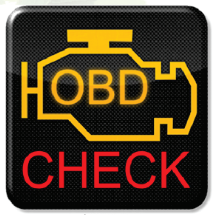
\includegraphics[width = 0.2\linewidth, height = 2cm]{Imagen_OBD-1.png}
		\caption{Imagen OBD-1.}
		\label{Imagen_OBD-1}
	\end{figure}
	\subsection{On Board Diagnostics II - OBD-2}\label{Etiqueta_Seccion_OBD2}
	OBD-2 es la segunda versión del OBD, que se modificó para encargarse también de monitorear el catalizador que afecta el nivel de emisiones del vehículo; para esto, se colocaron dos sondas que controlan el catalizador llamadas sondas
	lambda o sensores de oxígeno. \\\newline
	\indent Así como se encarga de revisar los componentes que afecten las emisiones de contaminantes, también manda una señal de alerta cuando ocurre alguna falla en el vehículo; el símbolo que marca el tablero, la señal de Check Engine, es el aviso que manda la computadora como alerta de alguna falla y, por lo tanto, sugiere llevar la unidad, lo más pronto posible, al taller mecánico. Además, el sistema OBDII guarda el registro de la falla al momento y ayuda al mecánico a determinar el porqué de esta \cite{CONUEE}. La Figura \ref{Parametros_OBD-2} muestra algunos de los parámetros que puede abarcar el lector OBD-2 y en la Figura \ref{Imagen_OBD-2} un ejemplo de lector OBD-2.
	\begin{figure}[!h]
		\centering
		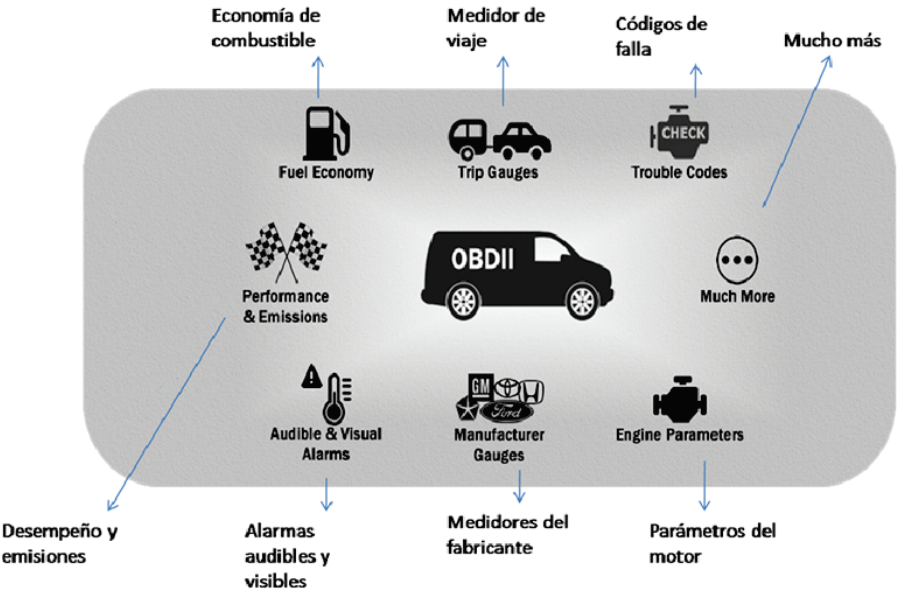
\includegraphics[width = 1\linewidth, height = 6.2cm]{Parametros_OBD-2.png}
		\caption{Algunos Parámetros sensor OBD-2.}
		\label{Parametros_OBD-2}
	\end{figure}
	\begin{figure}[!h]
		\centering
		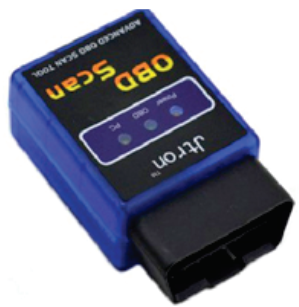
\includegraphics[width = 0.2\linewidth, height = 2cm]{Imagen_OBD-2.png}
		\caption{Imagen OBD-2.}
		\label{Imagen_OBD-2}
	\end{figure}
	
	\section{Almacenamiento de datos seguro en la nube - AWS S3}\label{Etiqueta_AWS_S3}
	Amazon Simple Storage Service (Amazon S3) es un servicio de almacenamiento de objetos que ofrece escalabilidad, disponibilidad de datos, seguridad y rendimiento líderes en el sector. Clientes de todos los tamaños y sectores pueden almacenar y proteger cualquier cantidad de datos para prácticamente cualquier caso de uso, como los lagos de datos, las aplicaciones nativas en la nube y las aplicaciones móviles. Gracias a las clases de almacenamiento rentables y a las características de administración fáciles de usar, es posible optimizar los costos, organizar los datos y configurar controles de acceso detallados para cumplir con requisitos empresariales, organizacionales y de conformidad específicos \cite{AWS_S3}. La Figura \ref{Funcionamiento_AWS_S3} muestra el funcionamiento de AWS S3.
	\begin{figure}[!h]
		\centering
		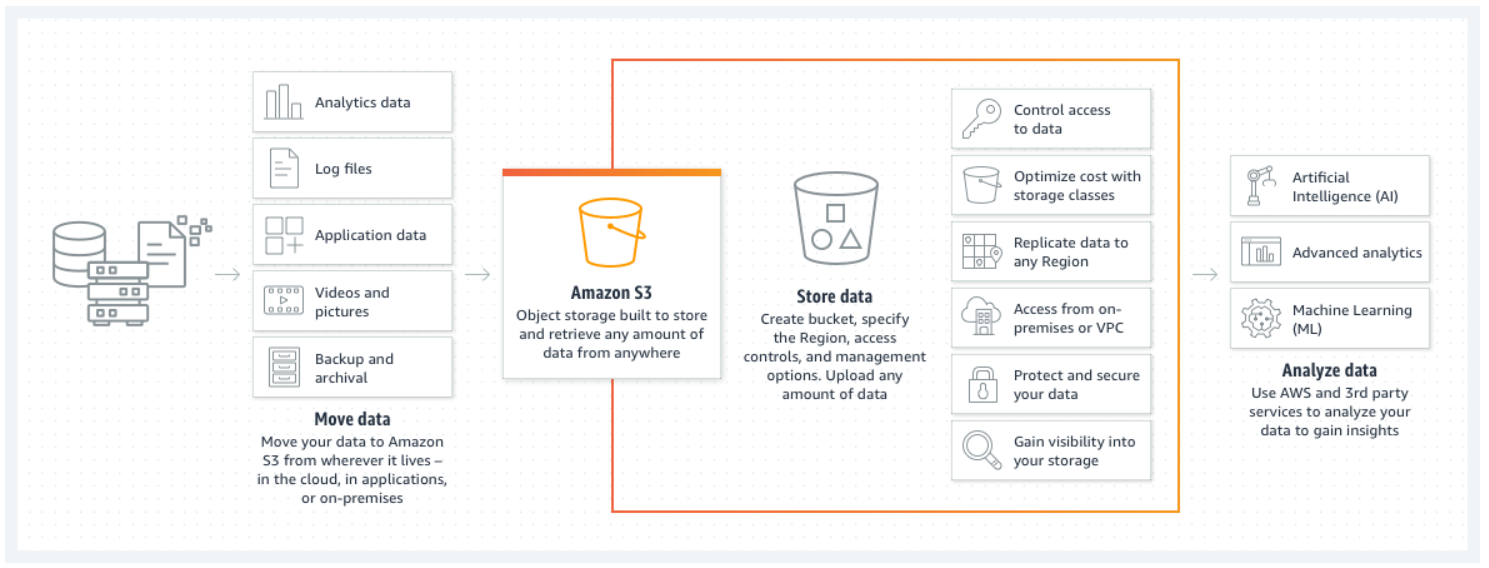
\includegraphics[width = 1\linewidth, height = 6.3cm]{Funcionamiento_AWS_S3.png}
		\caption{Funcionamiento de AWS S3.}
		\label{Funcionamiento_AWS_S3}
	\end{figure}
	
	\section{Implementación OBD-2 en APP Móvil - Android Studio}\label{Android_Studio_OBD}
	La implementación de una aplicación móvil en Android Studio implica un proceso completo de desarrollo que abarca desde la concepción de la idea hasta la entrega final del producto. Android Studio, siendo el entorno de desarrollo oficial respaldado por Google, juega un papel central en este proceso, proporcionando herramientas poderosas y funcionalidades que facilitan la creación de aplicaciones Android robustas y efectivas \cite{Android}. \\\newline
	\indent El primer paso en la implementación de una aplicación es la configuración del entorno de desarrollo. Esto implica descargar e instalar Android Studio, así como configurar el entorno con los componentes necesarios, como los paquetes de desarrollo de software (SDK) y las herramientas específicas de Android. Este paso es crucial para garantizar que el desarrollador tenga acceso a las bibliotecas y recursos necesarios para construir y probar la aplicación de manera efectiva.
	\subsection{Implementación Servicios de OBD-2}\label{Etiqueta_Implementacion_Servicios_OBD-2}
	Para la implementación de los servicios de OBD-2 dentro de la APP ``SIGOAVE'' es necesario seguir una secuencia de pasos que se describen a continuación:
	\begin{itemize}
		\item Modificación del archivo AndroidManifest.xml.
		\item Modificación del archivo build.gradle (Module:app).
		\item Modificación del archivo build.gradle (Project:SIGOAVE).
		\item Modificación del archivo string..xml.
		\item Creación de una actividad Parámetros y su clase.
		\item Creación de una clase tipo enumeración.
		\item Creación de una actividad OBD y su clase.
		\item Programación de la nueva actividad OBD.
	\end{itemize}
	\indent\newline\indent El primer paso a realizar es la modificación del archivo ``AndroidManifest.xml'' de la APP. En este archivo se agregaran los permisos necesarios para la implementación de los nuevos servicios. La Figura \ref{Permisos_APP_OBD} muestra los nuevos permisos agregados a la aplicación móvil.
	\begin{figure}[!h]
		\centering
		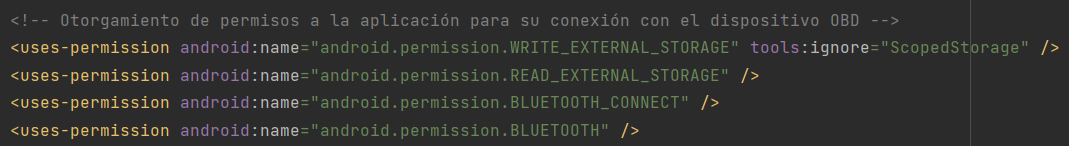
\includegraphics[width = 1\linewidth, height = 3.8cm]{Permisos_APP_OBD.png}
		\caption{Nuevos Permisos Servicios OBD.}
		\label{Permisos_APP_OBD}
	\end{figure} \\
	\indent En el segundo paso, se procede procede a agregar las dependencias de los servicios a utilizar en el archivo ``build.gradle (Module:app'' como se muestra en la Figura \ref{Nuevas_Dependencias_OBD}.
	\begin{figure}[!h]
		\centering
		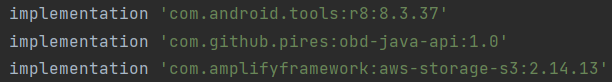
\includegraphics[width = 1\linewidth, height = 2.2cm]{Nuevas_Dependencias_OBD.png}
		\caption{Nuevas Dependencias OBD.}
		\label{Nuevas_Dependencias_OBD}
	\end{figure} \\
	\indent El tercer paso, se debe modificar el archivo ``Modificación archivo build.gradle (Project:SIGOAVE)'' en el cual se agregaran nuevos repositorios, plugins y tareas como muestra la Figura \ref{Nuevas_Tareas_OBD}.
	\begin{figure}[!h]
		\centering
		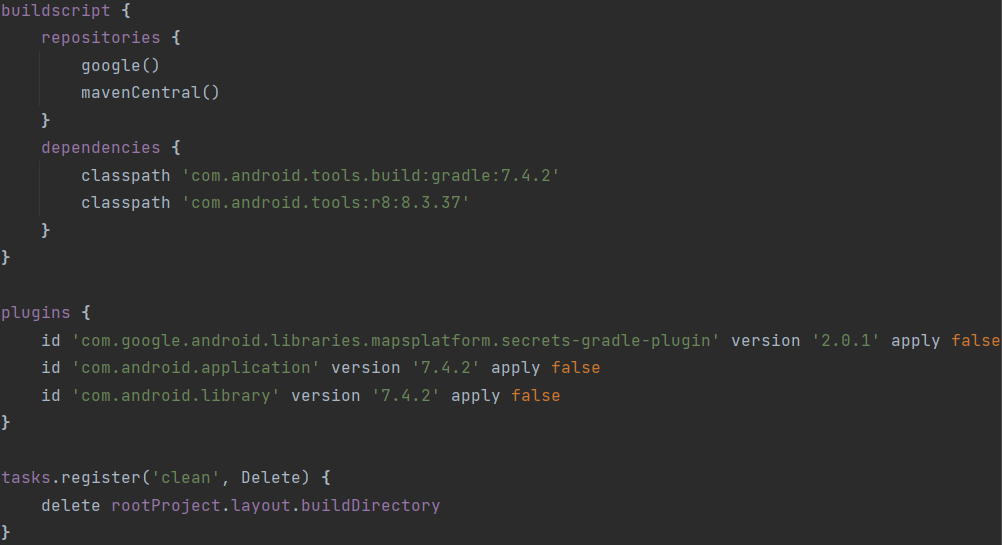
\includegraphics[width = 1\linewidth, height = 8.5cm]{Nuevas_Tareas_OBD.png}
		\caption{Nuevas Dependencias, Plugins y Tareas de OBD.}
		\label{Nuevas_Tareas_OBD}
	\end{figure} \\
	\indent En el cuarto paso, se debe modificar el archivo ``string..xml'', en el cual se agregaran las cadenas de texto a presentar dentro de la nueva actividad y dentro de los mensajes de alerta. La Figura \ref{String_Nuevo_OBD}.
	\begin{figure}[!h]
		\centering
		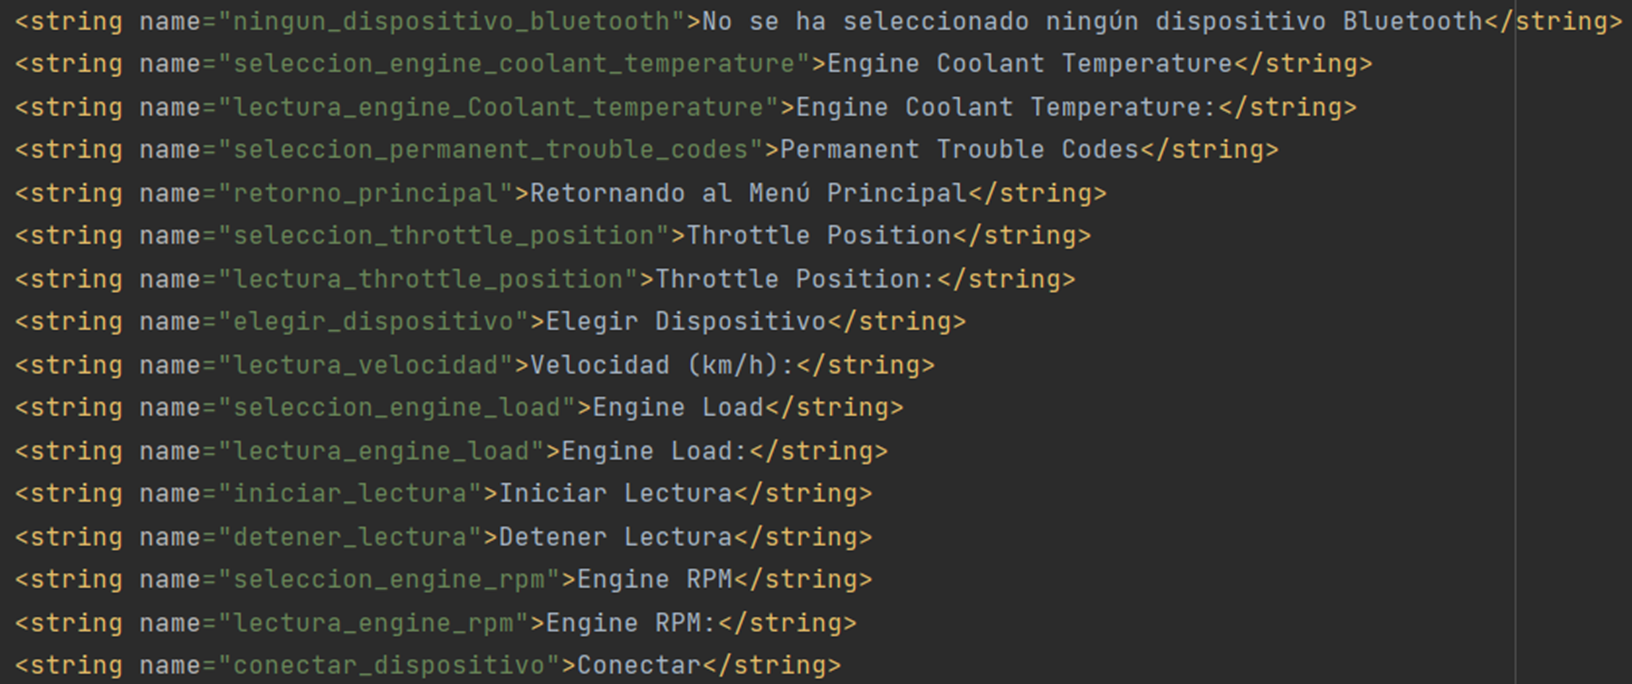
\includegraphics[width = 1\linewidth, height = 8.5cm]{String_Nuevo_OBD.png}
		\caption{Nuevas Cadenas de Texto.}
		\label{String_Nuevo_OBD}
	\end{figure} \\
	\indent Como quinto paso, se debe crear una nueva actividad y su respectiva clase. La clase y su actividad se llamara ``ParametrosActivity.java'' como muestra la Figura \ref{Parametros_Activity} y en la Figura \ref{Codigo_Parametros_Activity} se muestra un segmento de código respecto a esta clase.
	\begin{figure}[!h]
		\centering
		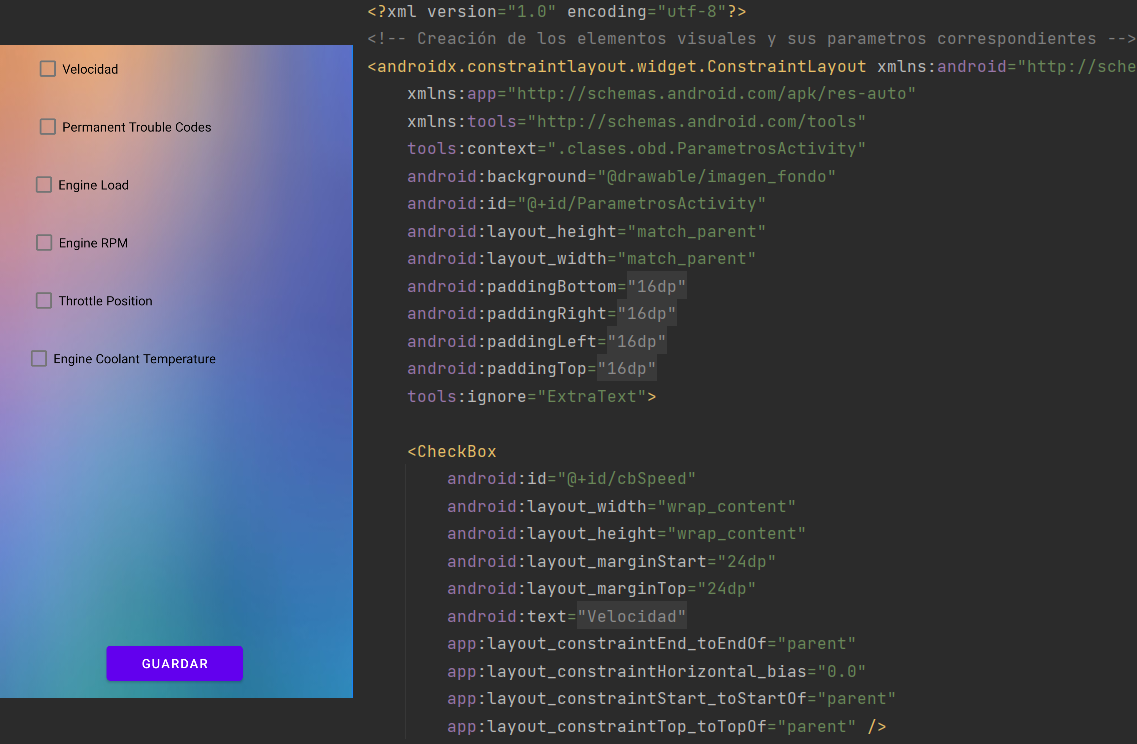
\includegraphics[width = 1\linewidth, height = 8.2cm]{Parametros_Activity.png}
		\caption{Segmento de Código de la Actividad de Parámetros.}
		\label{Parametros_Activity}
	\end{figure}
	\begin{figure}[!h]
		\centering
		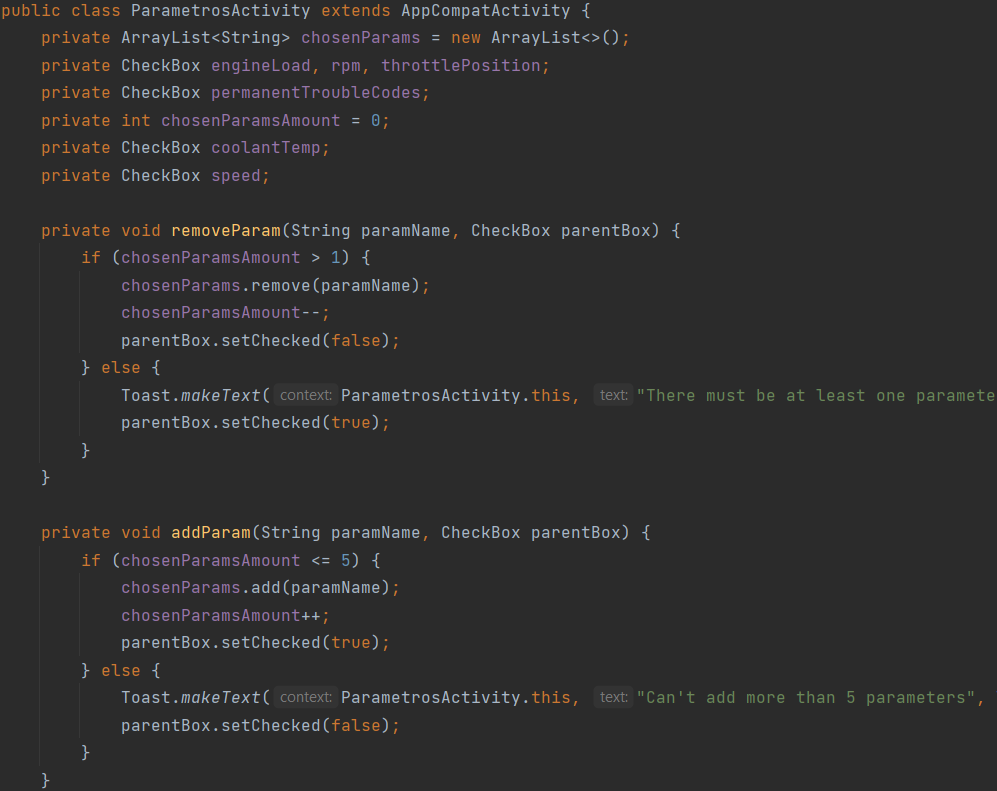
\includegraphics[width = 1\linewidth, height = 8.2cm]{Codigo_Parametros_Activity.png}
		\caption{Segmento de Código de la clase Parámetros.}
		\label{Codigo_Parametros_Activity}
	\end{figure} \\
	\indent La actividad y la clase creada, mencionadas anteriormente, sirven para escoger los parámetros a utilizarse en el momento de la lectura y guardado de datos que se trata en el apartado \ref{Eltiqueta_Lectura_Guardado_OBD-2}. \\\newline
	\indent Como sexto paso, se requiere de la creación de una clase tipo ``Enumeration'' la cual me permite pasar y enumerar los parámetros escogidos por el usuario al momento de mostrar la información en pantalla. La Figura \ref{Enumeracion_Parametros_OBD} muestra el código desarrollado en esta clase.
	\begin{figure}[!h]
		\centering
		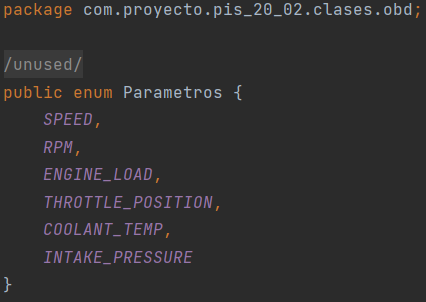
\includegraphics[width = 0.75\linewidth, height = 2.5cm]{Enumeracion_Parametros_OBD.png}
		\caption{Código de la clase Enumeración de Parámetros.}
		\label{Enumeracion_Parametros_OBD}
	\end{figure} \\
	\indent Como séptimo paso, corresponde al diseño de la interfaz grafica de la actividad principal de sistema de toma de datos por parte del lector OBD-2. En la Figura \ref{Interfaz_Grafica_OBD} se muestra la interfaz grafica diseñada y el segmento de código correspondiente a esta interfaz.
	\begin{figure}[!h]
		\centering
		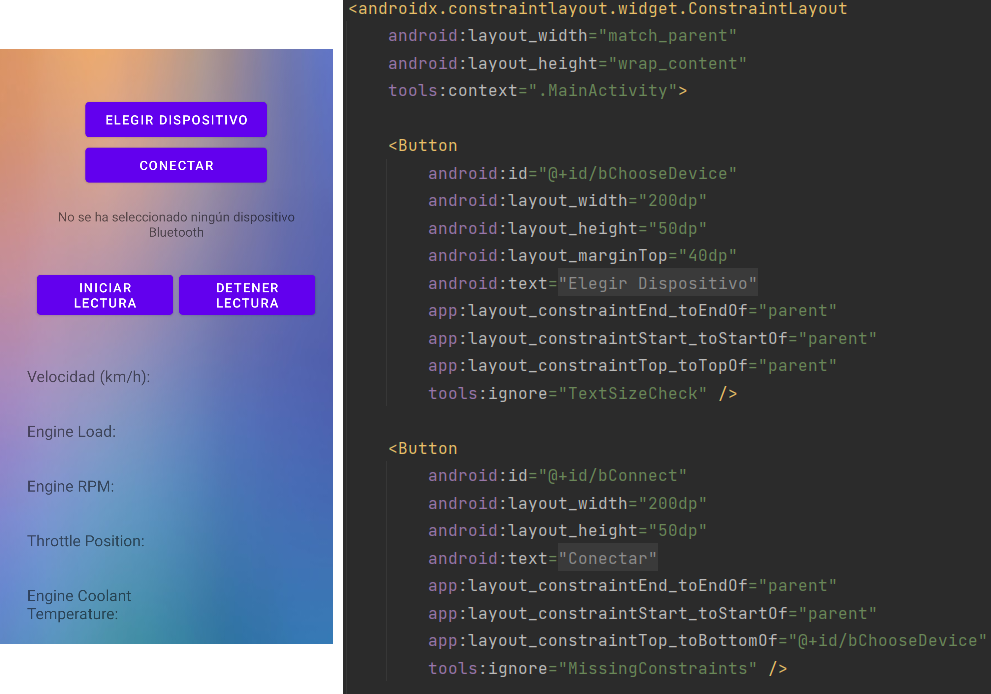
\includegraphics[width = 1\linewidth, height = 9.3cm]{Interfaz_Grafica_OBD.png}
		\caption{Interfaz Grafica de la Activity OBD.}
		\label{Interfaz_Grafica_OBD}
	\end{figure} \\
	\indent Una vez desarrollada la  interfaz grafica se debe modificar el archivo ``AndroidManifest.xml'' para que pueda haber una navegación fluida entre las diferentes actividades que comprende la APP. En la Figura \ref{Navegacion_OBD_Manifest}.
	\begin{figure}[!h]
		\centering
		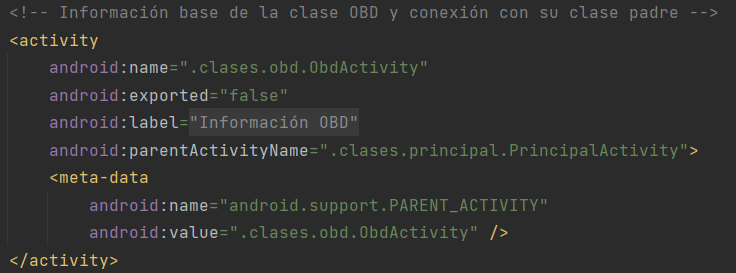
\includegraphics[width = 1\linewidth, height = 5cm]{Navegacion_OBD_Manifest.png}
		\caption{Control de Navegación OBD.}
		\label{Navegacion_OBD_Manifest}
	\end{figure} \\
	\indent Finalmente, como octavo paso se procede a la programación a la programación de la clase ``ObdActivity.java'' en la cual se encuentra toda lo lógica de negocios de lector OBD-2 con la APP. En esta clase se puede encontrar los métodos de conexión, búsqueda de dispositivos, lectura, almacenamiento de datos, entre otros. La Figura \ref{Logica_Negocios_OBD} muestra un segmento de código referente a la programación de esta clase.
	\begin{figure}[!h]
		\centering
		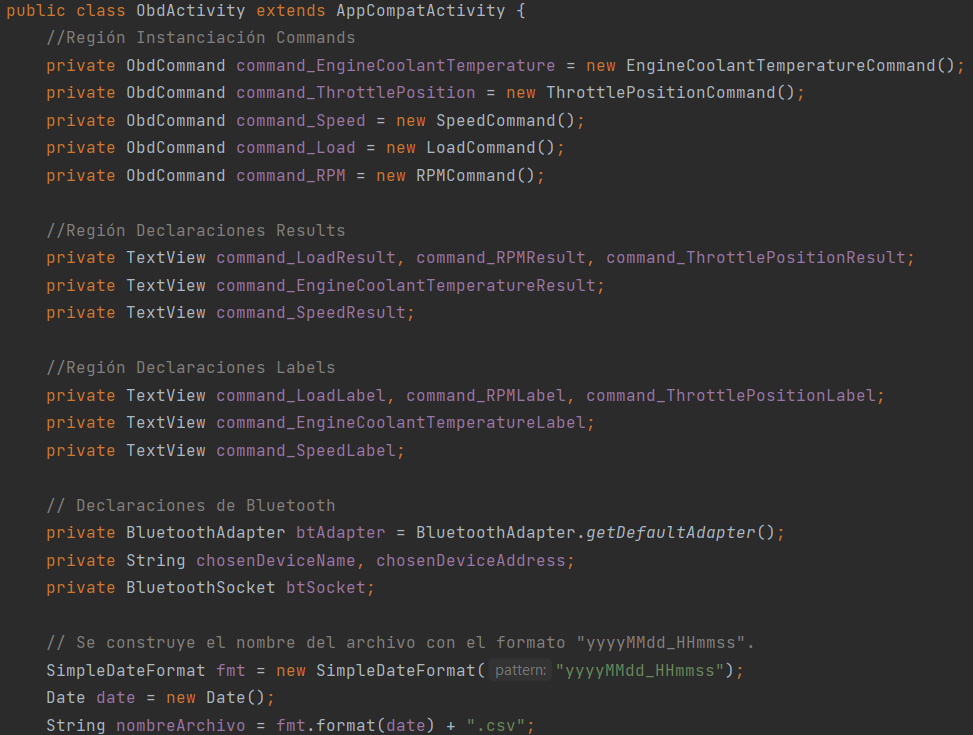
\includegraphics[width = 1\linewidth, height = 5.7cm]{Logica_Negocios_OBD.png}
		\caption{Lógica de Negocios Clase de OBD.}
		\label{Logica_Negocios_OBD}
	\end{figure}
	\subsection{Servicios AWS S3 para OBD-2}\label{Eltiqueta_Servicios_S3_AWS}
	Con la Interfaz Gráfica desarrollada y programada dentro de la APP, el siguiente paso es conectar la APP con los servicios de AWS. En este caso se hará uso de 3 servicios de AWS:
	\begin{itemize}
		\item AWS Amplify.
		\item AWS Cognito.
		\item AWS S3.
	\end{itemize}
	\indent\indent La información de la implementación de los dos primeros servicios (AWS Amplify y AWS Cognito) se encuentra explicado a detalle en el ``Manual de Instalación de Servicios en AWS para el Agente de Respuesta SIGOAVE''.  En el siguiente enlace se encuentra el Manual para su estudio:
	\begin{itemize}
		\item \textcolor{blue}{\url{https://github.com/laboratorioAI/PIS_20_02_AGENTES_IA/blob/main/Actualizacion_2024/Manual\%20Servicios\%20V1.0/Manual_Servicios.pdf}}
	\end{itemize}
	\indent\newline\indent Una vez que han sido creados los archivos de configuración mencionados en los puntos anteriores, el siguiente paso es añadir un espacio de almacenamiento para el proyecto en AWS, es decir, crear un bucket en AWS S3 dentro del cual se colocarán los archivos que se generen en el proyecto de Android. El comando que se utilizará para esto es: ``amplify add storage'', como se indica en la Figura \ref{AWS_Add_Storage}.
	\begin{figure}[!h]
		\centering
		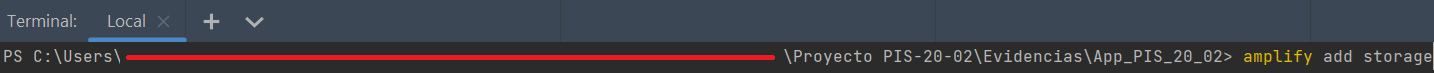
\includegraphics[width = 1\linewidth, height = 1cm]{AWS_Add_Storage.png}
		\caption{Comando S3 Agregar Almacenamiento.}
		\label{AWS_Add_Storage}
	\end{figure} \\
	\indent Una vez agregado el almacenamiento de datos, se procede con la configuración del ``Bucket de Almacenamiento''. En la Figura \ref{Configuracion_AWS_Bucket_S3} se muestra la configuración realizada.
	\begin{figure}[!h]
		\centering
		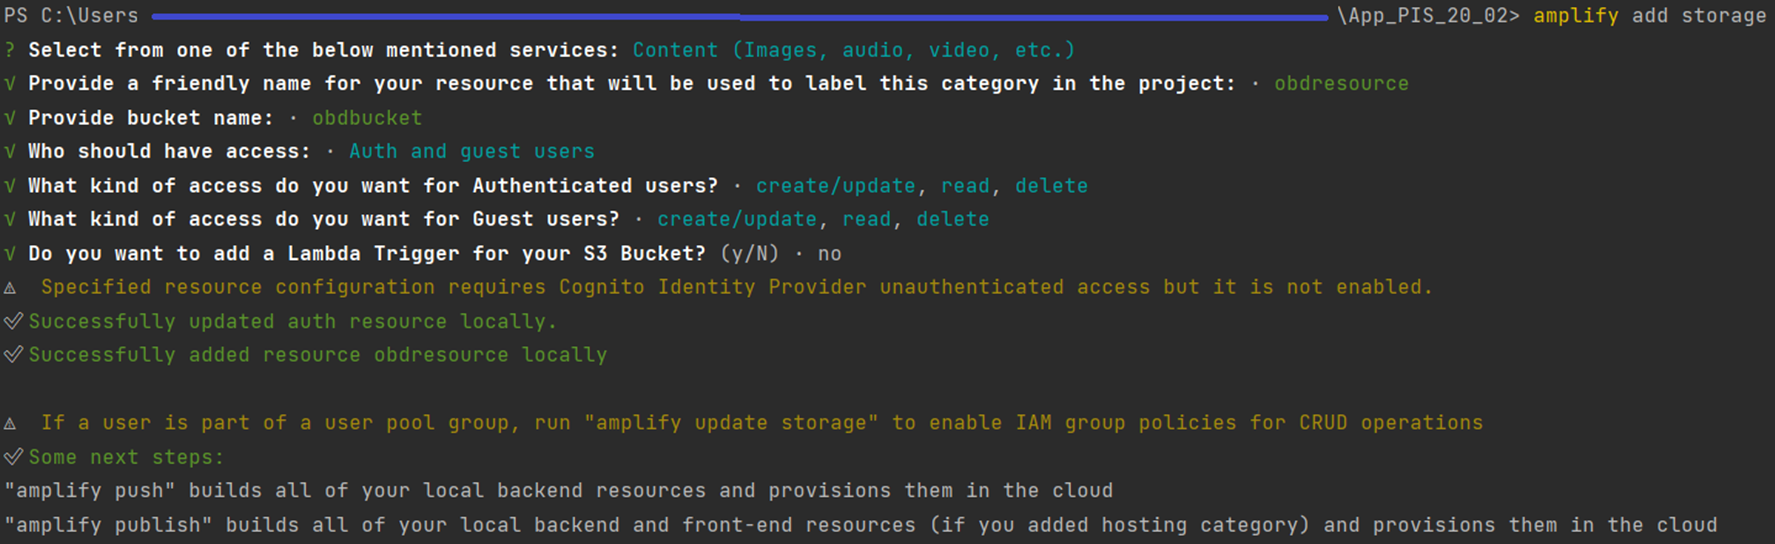
\includegraphics[width = 1\linewidth, height = 8.4cm]{Configuracion_AWS_Bucket_S3.png}
		\caption{Configuración AWS Bucket S3.}
		\label{Configuracion_AWS_Bucket_S3}
	\end{figure} \\
	\indent Después de realizar la configuración del ``Bucket de Almacenamiento'' se debe aplicar los cambios locales como remotos, para que estos sean persistentes en el tiempo mediante el comando: ``amplify push'' como muestra la Figura \ref{Amplify_Push_AWS_S3}.
	\begin{figure}[!h]
		\centering
		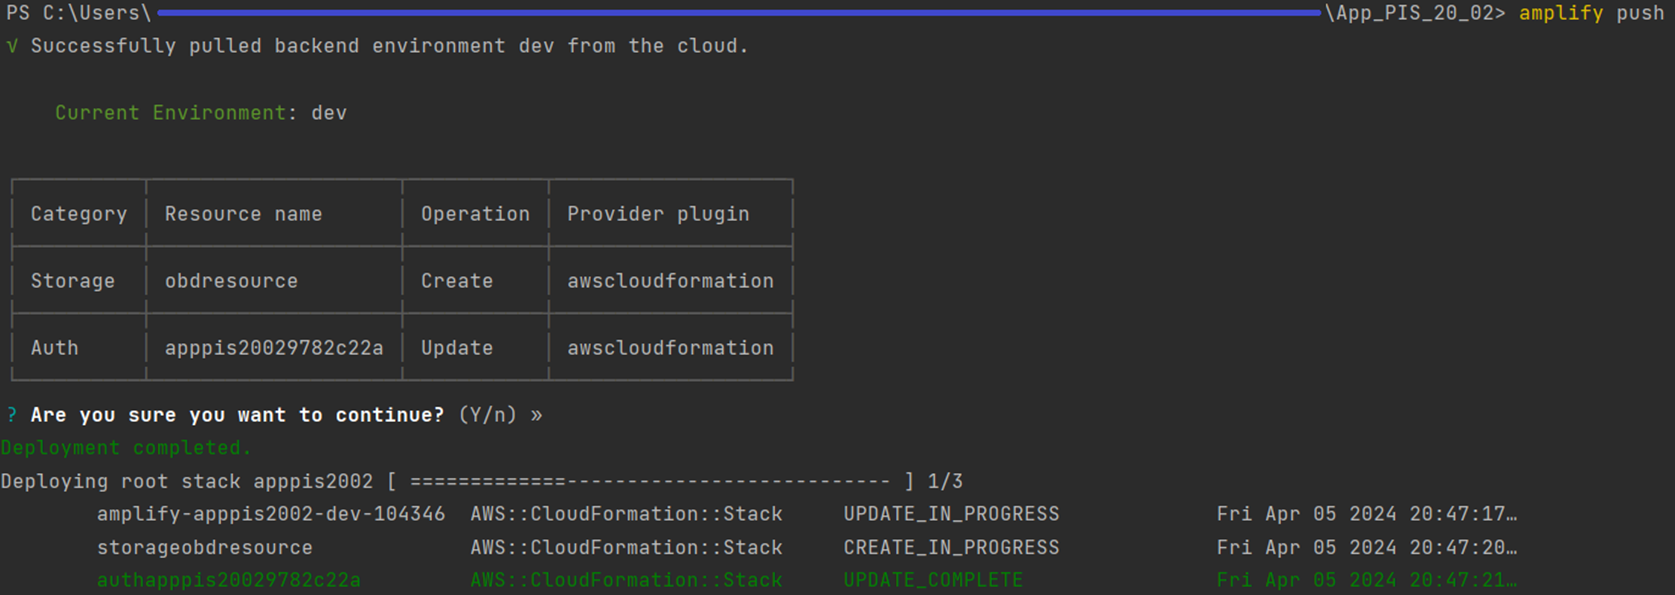
\includegraphics[width = 1\linewidth, height = 5.9cm]{Amplify_Push_AWS_S3.png}
		\caption{Amplify Push AWS S3.}
		\label{Amplify_Push_AWS_S3}
	\end{figure} \\
	\indent Al finalizar la ejecución del comando ``amplify push'', se puede observar que se ha creado un nuevo bucket llamado: 
	``obdbucket104346-dev'' en AWS, ver Figura \ref{Bucket_S3_Creado_OBD}.
	\begin{figure}[!h]
		\centering
		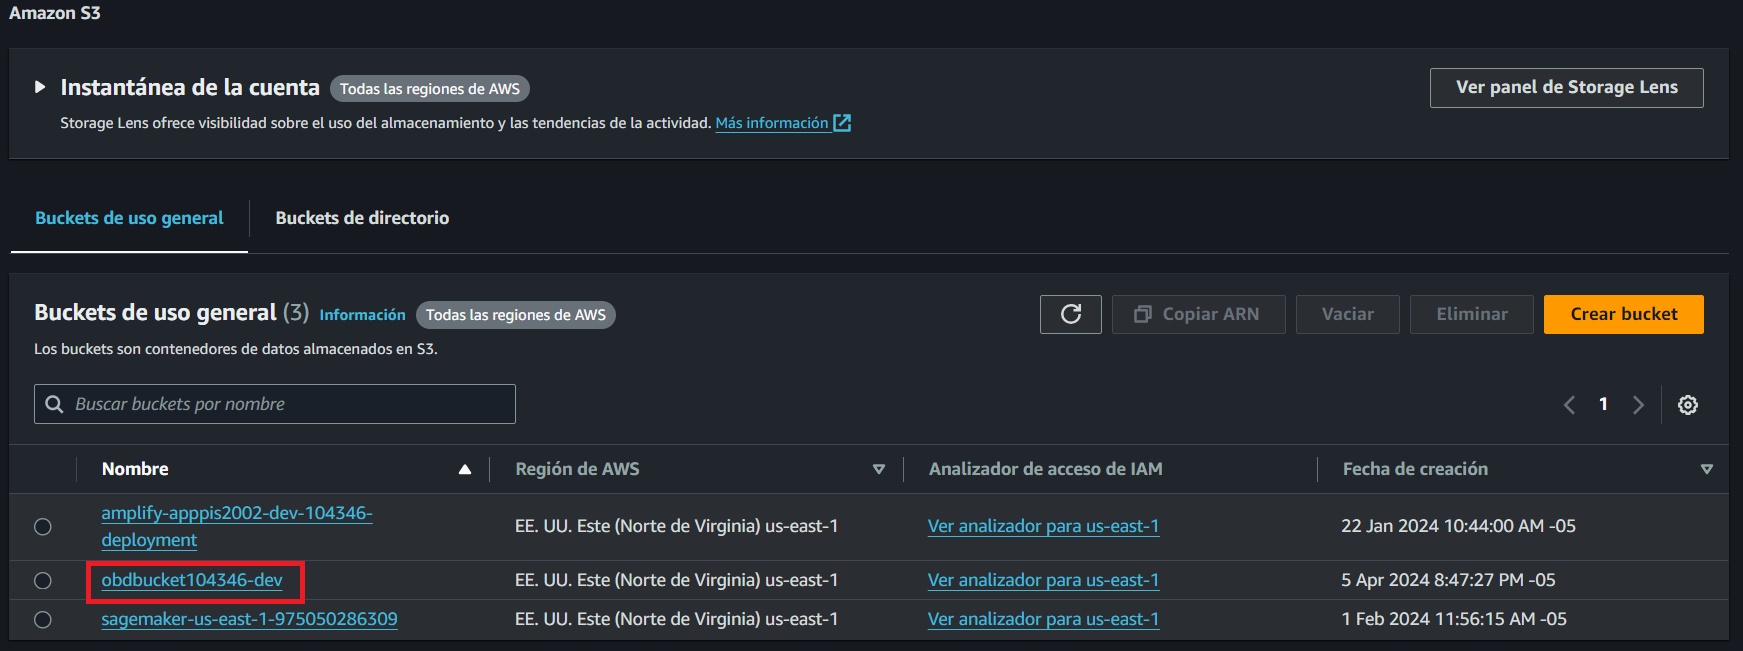
\includegraphics[width = 1\linewidth, height = 5.9cm]{Bucket_S3_Creado_OBD.png}
		\caption{Bucket OBD Creado en AWS S3.}
		\label{Bucket_S3_Creado_OBD}
	\end{figure}
	\subsection{Lectura y Guardado de datos por OBD-2}\label{Eltiqueta_Lectura_Guardado_OBD-2}
	Un lector OBD2 interpreta datos enviados por el sistema de diagnóstico de un vehículo moderno. Al conectar el lector al puerto OBD2 del automóvil, este dispositivo accede a una serie de parámetros que reflejan el estado del motor, emisiones y otros sistemas importantes. Al leer los datos, el lector OBD2 traduce códigos específicos, como códigos de falla, presión del combustible, temperatura del motor, velocidad del vehículo, entre otros, proporcionando así una visión detallada del rendimiento y la salud general del automóvil. La Figura \ref{Ejemplo_Dispositivo_OBD} muestra un ejemplo de un dispositivo OBD-2 \cite{CONUEE} de la marca VEEPAK.
	\begin{figure}[!h]
		\centering
		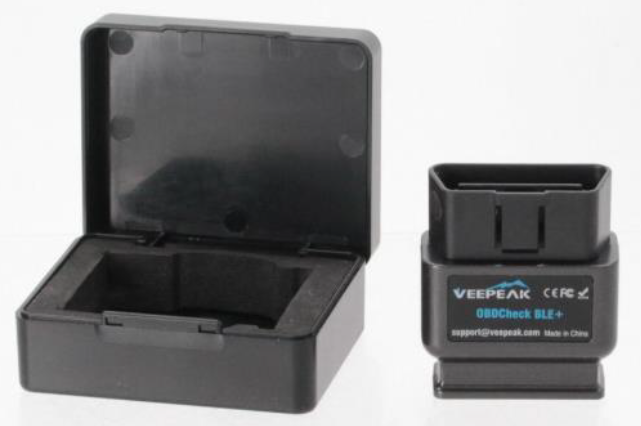
\includegraphics[width = 0.45\linewidth, height = 3cm]{Ejemplo_Dispositivo_OBD.png}
		\caption{Ejemplo de Dispositivo OBD-2.}
		\label{Ejemplo_Dispositivo_OBD}
	\end{figure} \\
	\indent De los diferentes parámetros con los cuales puede trabajar el lector OBD-2, se escogieron 5 parámetros esenciales para trabajar en la APP Móvil, estos son:
	\begin{itemize}
		\item Speed.
		\item Engine Load.
		\item RPM.
		\item Throtle Position.
		\item Engine Coolant Temperature.
	\end{itemize}
	\indent\indent En la Figura \ref{Flujo_Trabajo_OBD2} se muestra el flujo de trabajo de la aplicación, correspondiente a la obtención y almacenamiento de la información con los datos obtenidos desde el OBD-2.
	\begin{figure}[!h]
		\centering
		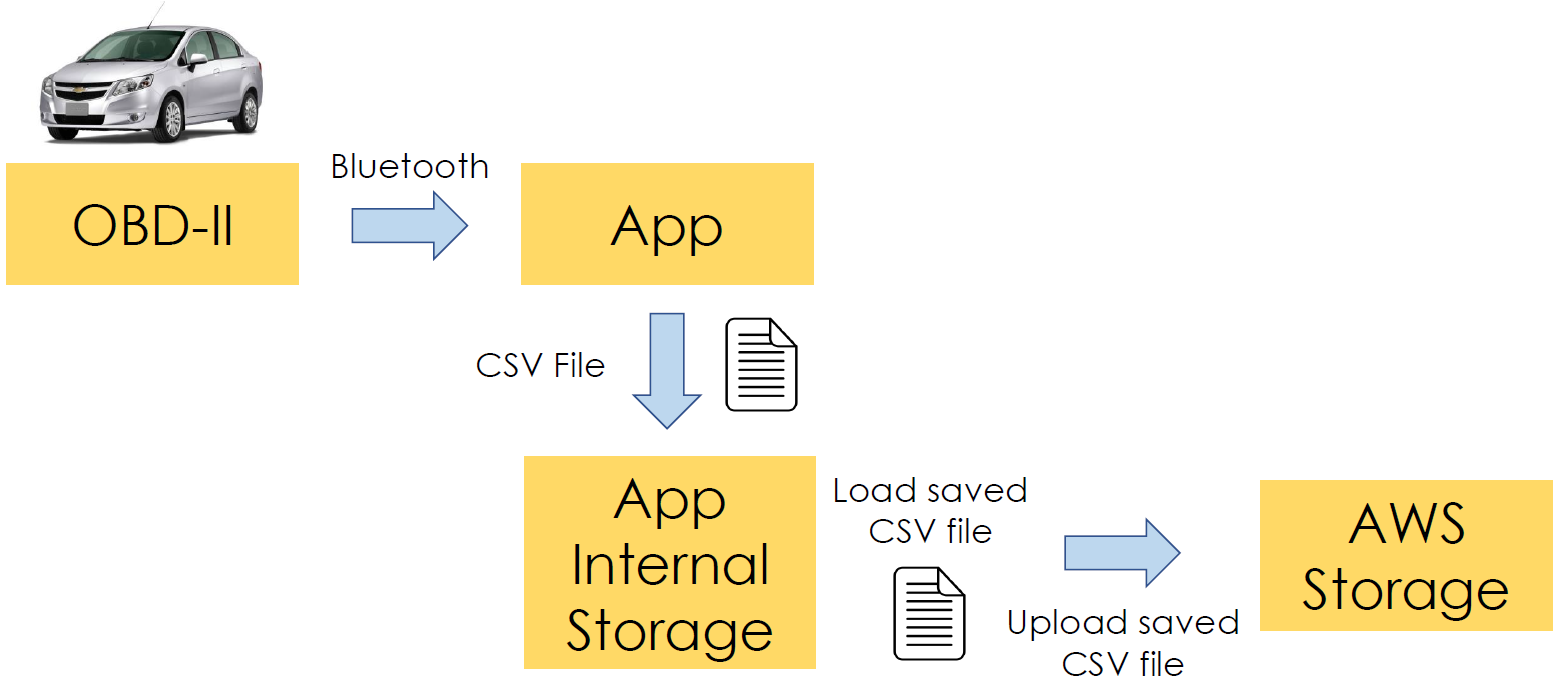
\includegraphics[width = 1\linewidth, height = 3cm]{Flujo_Trabajo_OBD2.png}
		\caption{Flujo de Trabajo de la Aplicación con OBD-2.}
		\label{Flujo_Trabajo_OBD2}
	\end{figure} \\
	\indent Finalmente, en la Figura \ref{Esquema_Funcionalidad_OBD} se muestra el esquema de funcionalidad del dispositivo OBD-2.
	\begin{figure}[!h]
		\centering
		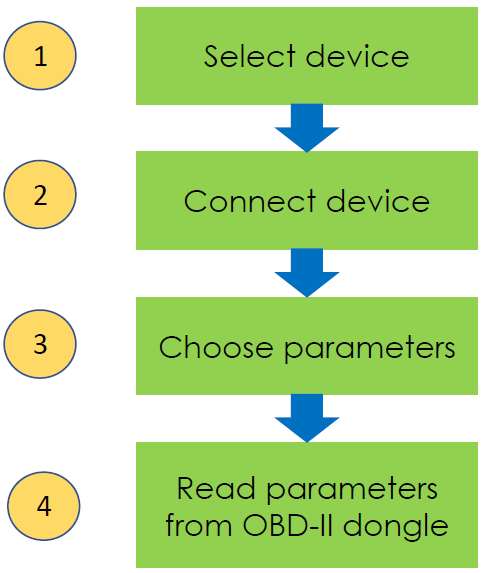
\includegraphics[width = 0.45\linewidth, height = 3.9cm]{Esquema_Funcionalidad_OBD.png}
		\caption{Esquema de Funcionalidad Dispositivo OBD-2.}
		\label{Esquema_Funcionalidad_OBD}
	\end{figure}

	\section{Prueba de Funcionamiento APP con OBD-2}\label{Prueba_Funcionamiento_OBD-2}
	Con la APP configurada, el siguiente paso es realizar las pruebas de funcionamiento de la APP móvil con el lector OBD-2 conectado al dispositivo. Para ello se debe abrir la aplicación desde el dispositivo móvil como muestra la Figura \ref{Apertura_App_OBD2}.
	\begin{figure}[!h]
		\centering
		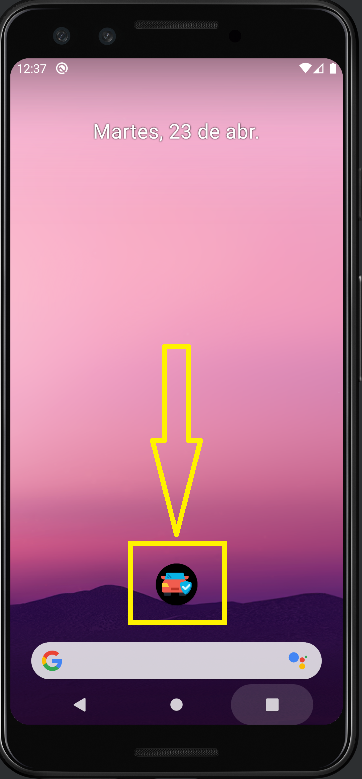
\includegraphics[width = 0.45\linewidth, height = 7.2cm]{Apertura_App_OBD2.png}
		\caption{Apertura de la APP desde el Dispositivo Móvil.}
		\label{Apertura_App_OBD2}
	\end{figure} \\
	\indent Una vez que se abre la APP se procede a registrarse o ingresar la credenciales, Ver Figura \ref{Registro_Ingreso_Credenciales}. Si previamente ya se ha iniciado sesión en el dispositivo móvil ya no es necesario volver a ingresar las credenciales.
	\begin{figure}[!h]
		\centering
		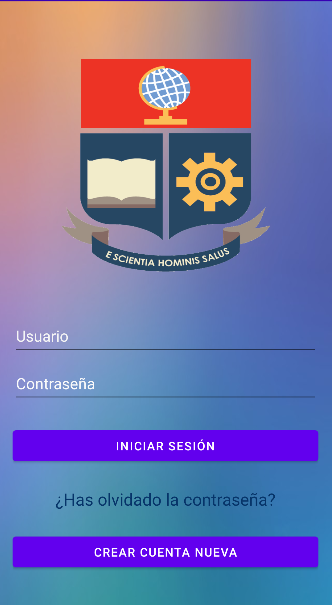
\includegraphics[width = 0.45\linewidth, height = 7.2cm]{Registro_Ingreso_Credenciales.png}
		\caption{Panel de Inicio de Sesión.}
		\label{Registro_Ingreso_Credenciales}
	\end{figure} \\
	\indent Si se desea crear un nuevo usuario se debe revisar el manual de usuario de la aplicación que se encuentra alojado en GitHub. En el siguiente enlace se encuentra el manual de usuario de la APP:
	\begin{itemize}
		\item \textcolor{blue}{\url{https://github.com/laboratorioAI/PIS_20_02_AGENTES_IA/tree/main/Actualizacion_2024/Manual\%20V3.0}}
	\end{itemize}
	\indent\indent Una vez dentro de la APP se debe dirigir a la sección del lector OBD-2 como indica la Figura \ref{Seccion_OBD2}, lo cual abrirá un nuevo panel dentro de la aplicación móvil.
	\begin{figure}[!h]
		\centering
		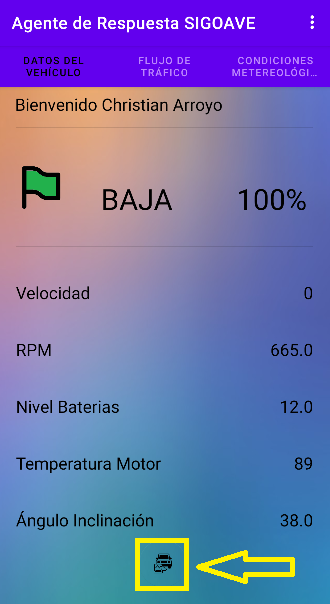
\includegraphics[width = 0.45\linewidth, height = 5.8cm]{Seccion_OBD2.png}
		\caption{Sección de inicio de OBD-2.}
		\label{Seccion_OBD2}
	\end{figure} \\
	\indent La Figura \ref{Informacion_OBD2}, muestra el panel del dispositivo de lectura OBD-2. En este panel se puede escoger el dispositivo OBD-2 que se encuentra conectado al vehículo y el mismo que sera conectado a la aplicación móvil. Al presionar sobre la opción ``Eligir Dispositivo'' se desplegara la lista de dispositivos OBD-2 disponibles, ver Figura \ref{Lista_Dispositivos_OBD2}, se deberá escoger el dispositivo que se encuentra conectado al vehículo al cual se desea tomar las mediciones.
	\begin{figure}[!h]
		\centering
		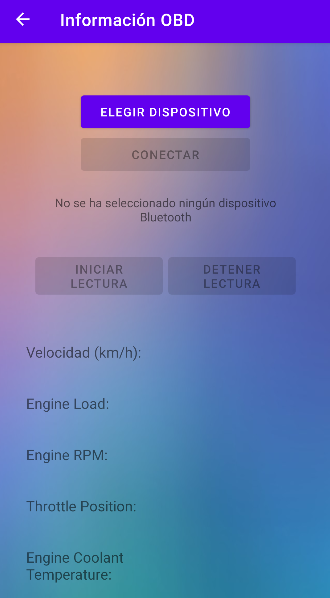
\includegraphics[width = 0.45\linewidth, height = 5.8cm]{Informacion_OBD2.png}
		\caption{Panel de Información de OBD-2.}
		\label{Informacion_OBD2}
	\end{figure}
	\begin{figure}[!h]
		\centering
		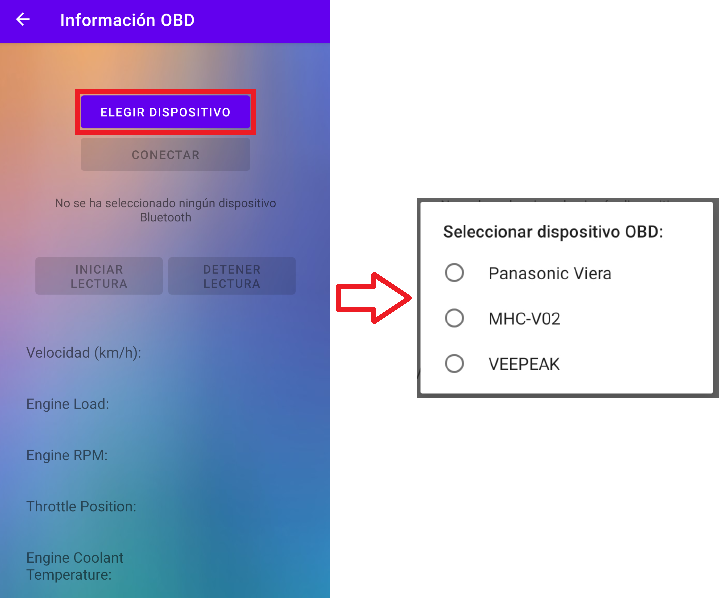
\includegraphics[width = 0.7\linewidth, height = 8.3cm]{Lista_Dispositivos_OBD2.png}
		\caption{Lista de Dispositivos OBD-2.}
		\label{Lista_Dispositivos_OBD2}
	\end{figure} \\
	\indent Una vez seleccionado el dispositivo se regresara al panel principal de información OBD-2, donde se puede apreciar que el botón ``Conectar'' se encuentra habilitado y se muestra información relevante sobre el dispositivo seleccionado (nombre y dirección del dispositivo), ver Figura \ref{Dispositivo_OBD2_Seleccionado}.
	\begin{figure}[!h]
		\centering
		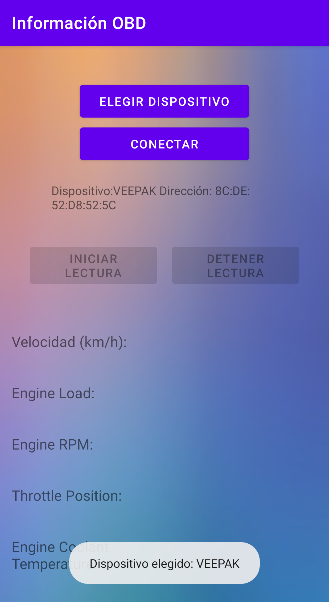
\includegraphics[width = 0.45\linewidth, height = 8.3cm]{Dispositivo_OBD2_Seleccionado.png}
		\caption{Dispositivo OBD-2 Seleccionado.}
		\label{Dispositivo_OBD2_Seleccionado}
	\end{figure} \\
	\indent Posteriormente se procede a conectar el dispositivo con la aplicación para lo cual se presiona el botón ``Conectar'', tras lo cual se mostrará un mensaje de alerta en el cual se informa el estado de la conexión, ver Figura \ref{Conectar_OBD-2}.
	\begin{figure}[!h]
		\centering
		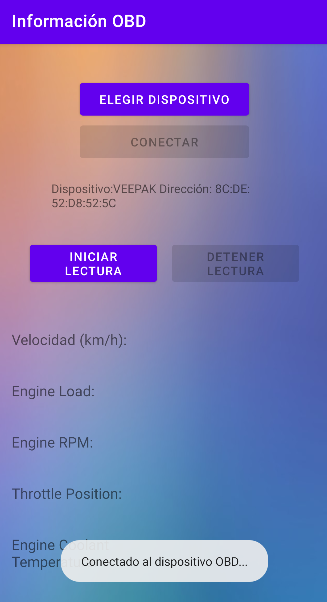
\includegraphics[width = 0.45\linewidth, height = 7.6cm]{Conectar_OBD-2.png}
		\caption{Conexión con Dispositivo OBD-2.}
		\label{Conectar_OBD-2}
	\end{figure} \\
	\indent Tras conectar el dispositivo OBD-2 a la APP se aprecia en el panel principal que el botón ``Conectar'' se encuentra deshabilitado y el botón ``Iniciar Lectura'' se encuentra habilitado. El botón ``Iniciar Lectura'' permite iniciar con la lectura de las mediciones del vehículo tras presionar este botón, ver Figura \ref{Inicio_Mediciones_OBD-2}.
	\begin{figure}[!h]
		\centering
		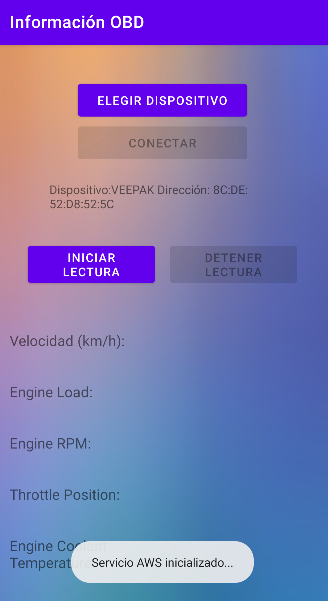
\includegraphics[width = 0.45\linewidth, height = 7.6cm]{Inicio_Mediciones_OBD-2.png}
		\caption{Inicio de Mediciones Dispositivo OBD-2.}
		\label{Inicio_Mediciones_OBD-2}
	\end{figure} \\
	\indent Al iniciar con la lectura de datos del vehículo, el dispositivo establecerá conexión con los servicios de AWS S3, explicados en el apartado \ref{Etiqueta_AWS_S3}. Esto permitirá almacenar la información de forma segura en la nube para su posterior tratamiento. En la Figura \ref{Presentacion_Almacenamiento_Lecturas_OBD} muestra las lecturas tomadas por el lector OBD-2, estas lecturas son tomadas cada 5 segundos y son enviadas internamente a los servicios de AWS S3. Adicionalmente, se aprecia que una serie de botones se encuentran deshabilitados para evitar conexiones con otros dispositivos y que el botón ``Detener Lectura'' se encuentra habilitado. Ver Figura \ref{Presentacion_Almacenamiento_Lecturas_OBD}.
	\begin{figure}[!h]
		\centering
		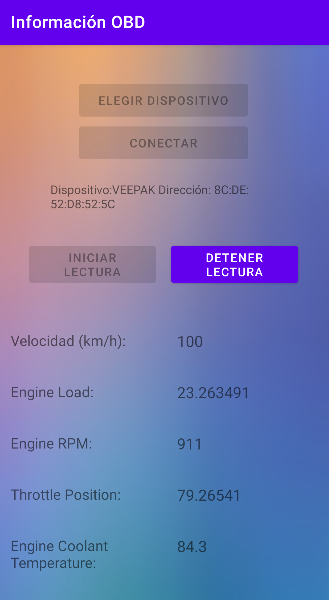
\includegraphics[width = 0.45\linewidth, height = 6.7cm]{Presentacion_Almacenamiento_Lecturas_OBD.png}
		\caption{Presentación y Almacenamiento de Lecturas del Dispositivo OBD-2.}
		\label{Presentacion_Almacenamiento_Lecturas_OBD}
	\end{figure} \\
	\indent Al presionar el botón ``Detener Lectura'' el dispositivo OBD-2 dejara de enviar datos a la APP y todos los datos obtenidos se almacenaran en un archivo con extensión ``CSV'', ver Figura \ref{Datos_OBD_Guardados_CSV}.
	\begin{figure}[!h]
		\centering
		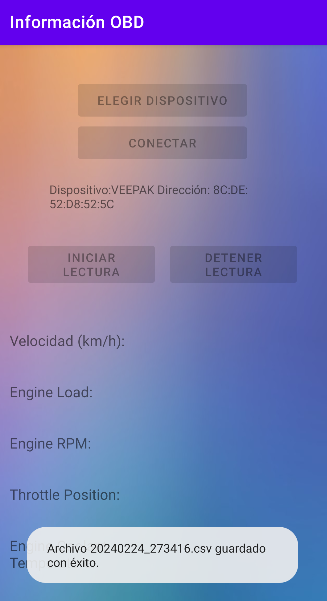
\includegraphics[width = 0.45\linewidth, height = 6.7cm]{Datos_OBD_Guardados_CSV.png}
		\caption{Datos Dispositivo OBD-2 Guardados en archivo CSV.}
		\label{Datos_OBD_Guardados_CSV}
	\end{figure} \\
	\indent Una vez que el archivo generado con los datos del vehículo se haya terminado de subir a la nube se mostrara un mensaje de alerta informando al usuario, ver Figura \ref{Archivo_CSV_OBD_Subido_S3}.
	\begin{figure}[!h]
		\centering
		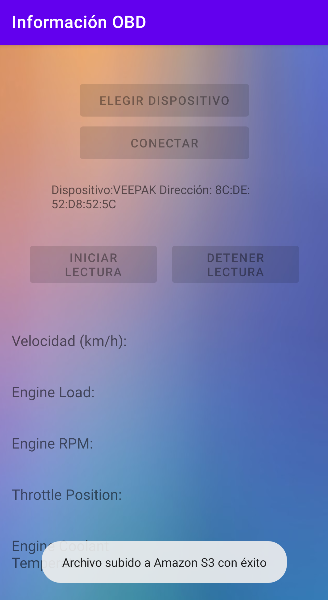
\includegraphics[width = 0.45\linewidth, height = 9cm]{Archivo_CSV_OBD_Subido_S3.png}
		\caption{Archivo CSV con Datos del Vehículo AWS S3.}
		\label{Archivo_CSV_OBD_Subido_S3}
	\end{figure} \\
	\indent  Luego de ejecutar la aplicación, al interior del bucket, se crea un directorio denominado ``public'', tal como se observa en la Figura \ref{Directorio_Public_S3_OBD}. Se debe recalcar que este directorio únicamente se crea la primera vez que se ejecuta la aplicación, a partir de la segunda ejecución, este directorio ya no se crea nuevamente, simplemente los archivos se almacenan en su interior.
	\begin{figure}[!h]
		\centering
		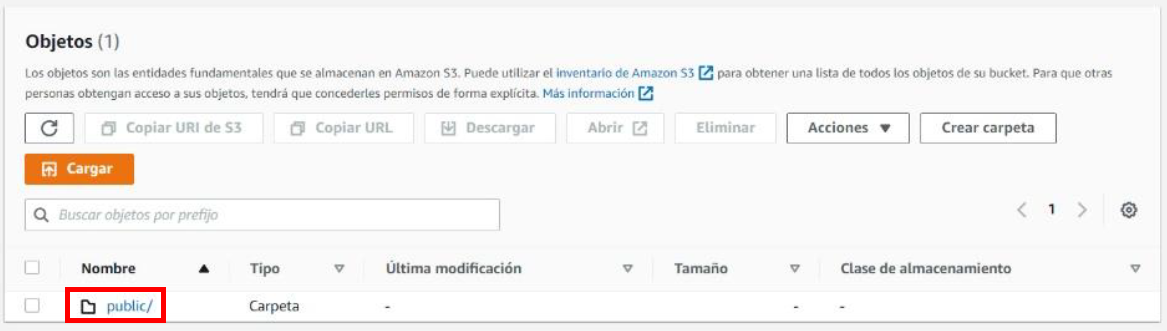
\includegraphics[width = 1\linewidth, height = 5.8cm]{Directorio_Public_S3_OBD.png}
		\caption{Directorio Public S3 OBD.}
		\label{Directorio_Public_S3_OBD}
	\end{figure} \\
	Finalmente, se puede observar que en el interior del directorio ``public'', han sido los almacenados los archivos creados por la aplicación ``SIGOAVE'', se puede verificar su existencia en los servicios de S3 en AWS como muestra la Figura \ref{Verificacion_Archivo_OBD_S3}. Aquí se puede observar todos los archivos generados mediante la APP en diferentes fechas los cuales contienen varias filas y columnas.
	\begin{figure}[!h]
		\centering
		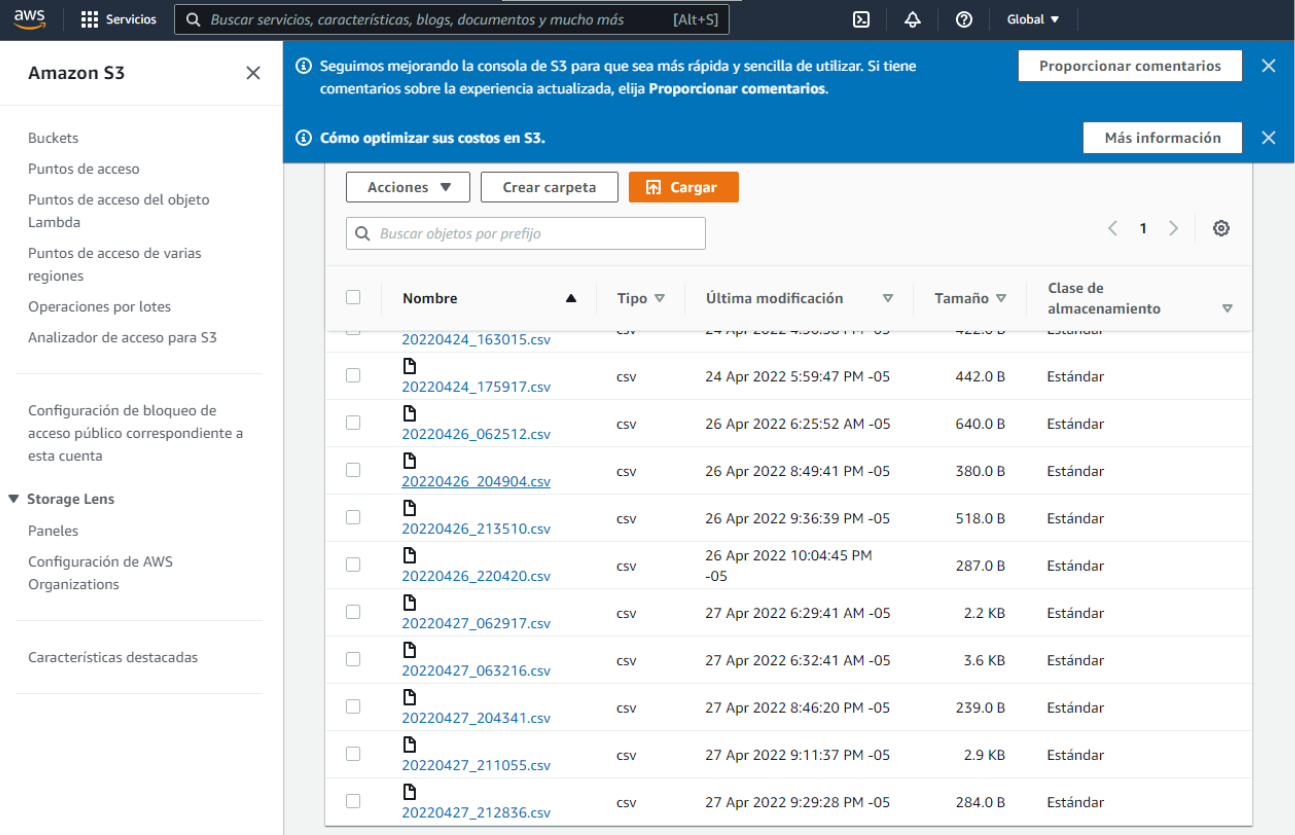
\includegraphics[width = 1\linewidth, height = 6cm]{Verificacion_Archivo_OBD_S3.png}
		\caption{Verificación de Archivos OBD en S3.}
		\label{Verificacion_Archivo_OBD_S3}
	\end{figure} \\
	\indent Si se desea, los archivos ``CSV'' alojados en los servicios de S3 pueden ser descargados al computador al dispositivo móvil para su uso. La Figura \ref{Descarga_CSV_OBD_S3} muestra el esquema de descarga de estos archivos y la Figura\ref{Ejemplo_Datos_OBD} muestra un ejemplo de los datos tomados por el lector OBD-2. 
	\begin{figure}[!h]
		\centering
		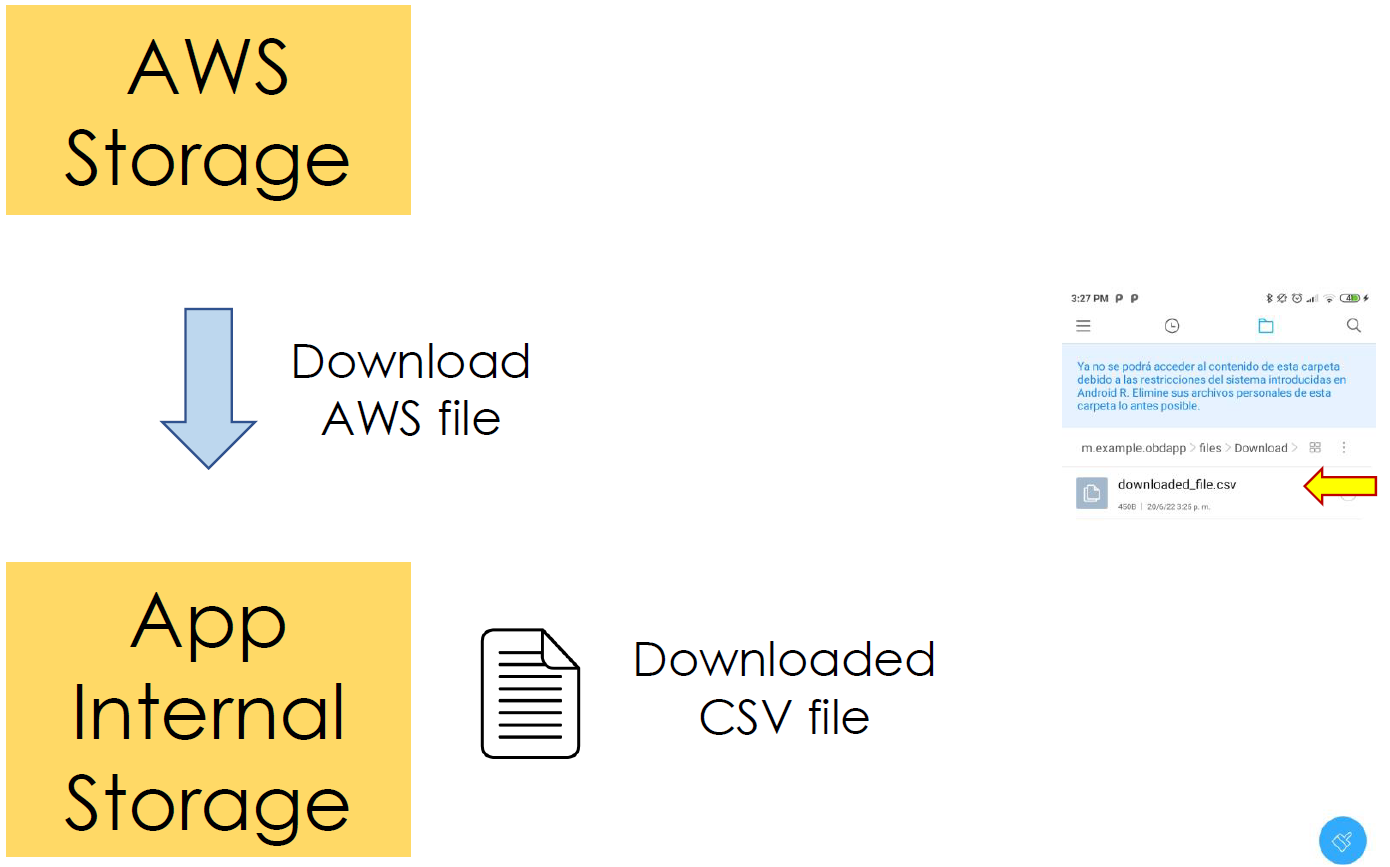
\includegraphics[width = 1\linewidth, height = 3.4cm]{Descarga_CSV_OBD_S3.png}
		\caption{Descarga Archivos CSV con Datos OBD desde S3.}
		\label{Descarga_CSV_OBD_S3}
	\end{figure}
	\begin{figure}[!h]
		\centering
		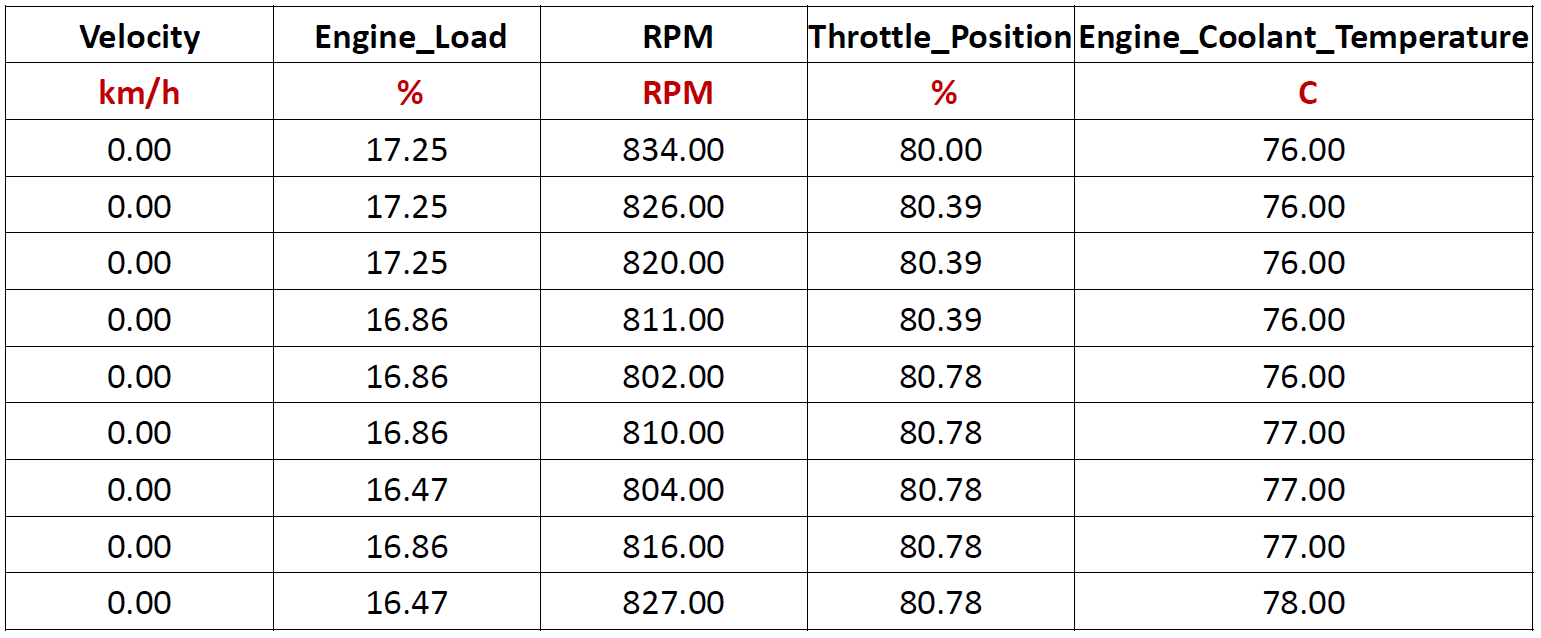
\includegraphics[width = 1\linewidth, height = 3.3cm]{Ejemplo_Datos_OBD.png}
		\caption{Ejemplo de Datos Lector OBD-2.}
		\label{Ejemplo_Datos_OBD}
	\end{figure}
	
	\section{Carga de Base de Datos en DynamoDB}\label{Etiqueta_Carga_Base_DyanmoDB}
	En este punto corresponde a carga una serie de base de datos a la base de datos de DynamoDB en AWS. Estas bases de datos servirá para su análisis y estudios futuros. Para cargar la base de datos en los servicios de AWS, el primer paso corresponde a crear un ``Bucket'' dentro de S3 en AWS. Como muestra la Figura \ref{Creacion_Nuevo_Bucket_S3}.
	\begin{figure}[!h]
		\centering
		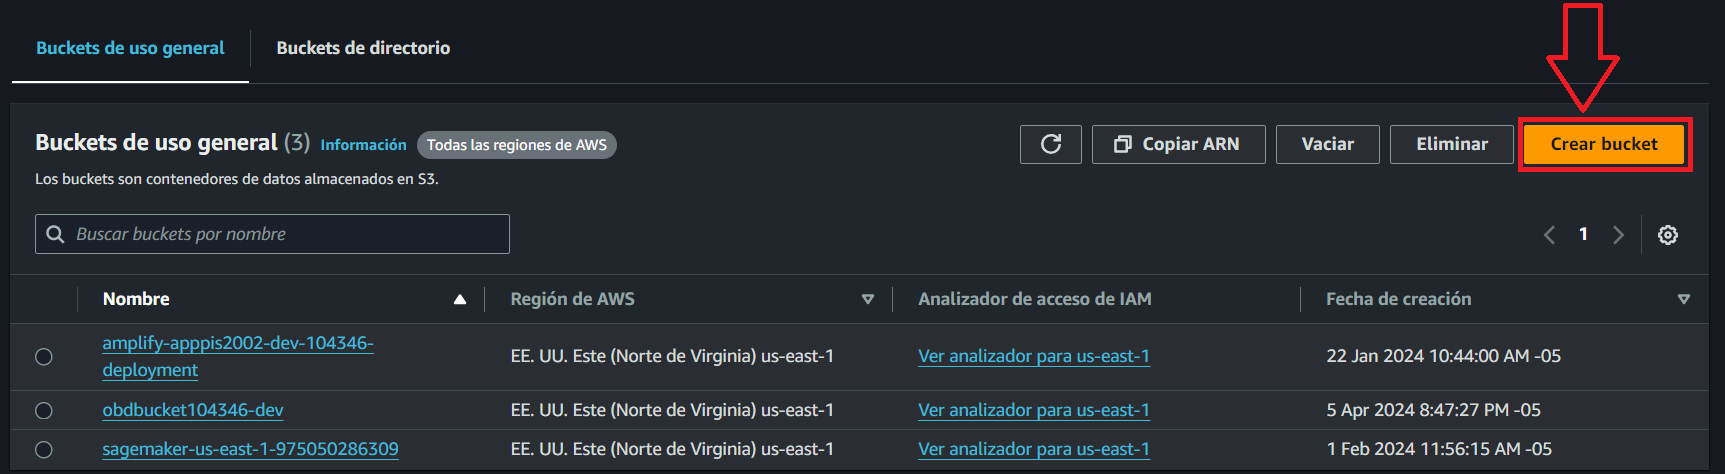
\includegraphics[width = 1\linewidth, height = 3.2cm]{Creacion_Nuevo_Bucket_S3.png}
		\caption{Creación de Nuevo Bucket en S3.}
		\label{Creacion_Nuevo_Bucket_S3}
	\end{figure} \\
	\indent Al nuevo bucket creado se le debe realizar una configuración básica (tipo, nombre, propiedades, etc.). La Figura \ref{Configuracion_Nuevo_Bucket_S3} muestra la configuración realizada al momento de crear el nuevo bucket. Al finalizar la configuración se debe presionar sobre el botón ``Crear bucket''. \\\newline
	\indent Tras crear el nuevo bucket, se retorna al panel de control principal de S3 donde se aprecia el nuevo bucket en la lista de ``Buckets de uso general''. Este procedimiento se lo realiza para todos los buckets que se va a usar en esta etapa. La Figura \ref{Todos_Nuevo_Bucket_S3} muestra la lista de todos los bucket creados. \\\newline
	\indent Una vez creado los bucket se procede a cargar los archivo que se van a utilizar en el bucket, en este caso serán las base de datos con extensión CSV. Para cargar los archivos primero se debe seleccionar el bucket, lo cual dirigirá al usuario a una nueva pantalla. En esta nueva pantalla se debe escoger la opción ``Cargar'' como muestra la Figura \ref{Carga_Archivo_CSV_Nuevo_Bucket}. \\\newline
	\indent Al seleccionar la opción ``Cargar'' se mostrara una nueva pantalla, en la cual permitirá al usuario agregar los archivos o carpetas que desee, como muestra la Figura \ref{Busqueda_Archivo_CSV_Bucket}. Al presionar sobre el botón ``Agregar Archivos'' se abrirá una ventana emergente la cual permite buscar en el dispositivo el archivo y seleccionarlo para su carga. Ver Figura \ref{Seleccion_Archivo_CSV_Bucket}. \\\newline
	\indent Una vez seleccionado el archivo, se regresa al pantalla de carga donde se aprecia el archivo seleccionado y el ``Destino'' que sera usado en el futuro para cargar la información dentro de DynamoDB. La Figura \ref{Archivo_Destino_Bucket_S3} muestra la configuración completa al cargar el archivo. En esta pantalla se debe proceder a presionar el botón ``Cargar'' en la parte inferior para iniciar con la carga del archivo dentro del bucket. \\\newline
	\indent Al Finalizar, se mostrara un mensaje informando al usuario el estado de la carga y si este tuvo errores o no. La Figura \ref{Carga_Completa_Archivo_Bucket} muestra la información completa al cargar el archivo. 
	\begin{figure}[!h]
		\centering
		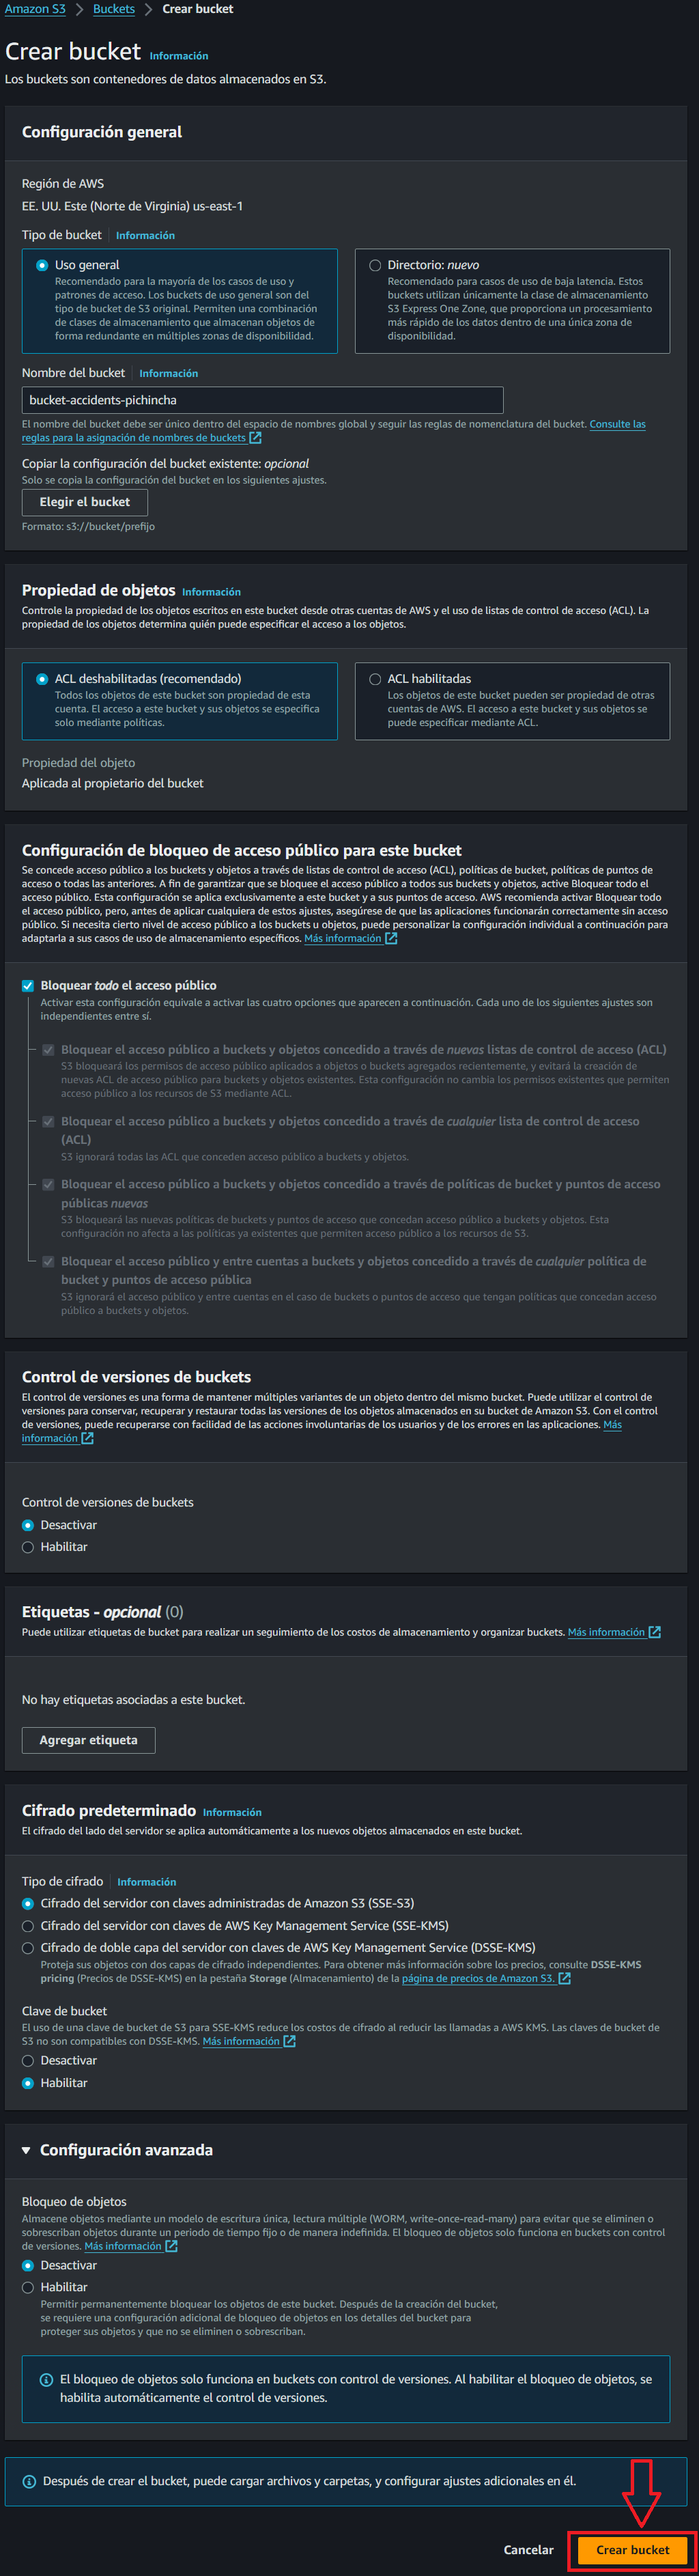
\includegraphics[width = 1\linewidth, height = 19.5cm]{Configuracion_Nuevo_Bucket_S3.png}
		\caption{Configuración del Nuevo Bucket S3.}
		\label{Configuracion_Nuevo_Bucket_S3}
	\end{figure}
	\begin{figure}[!h]
		\centering
		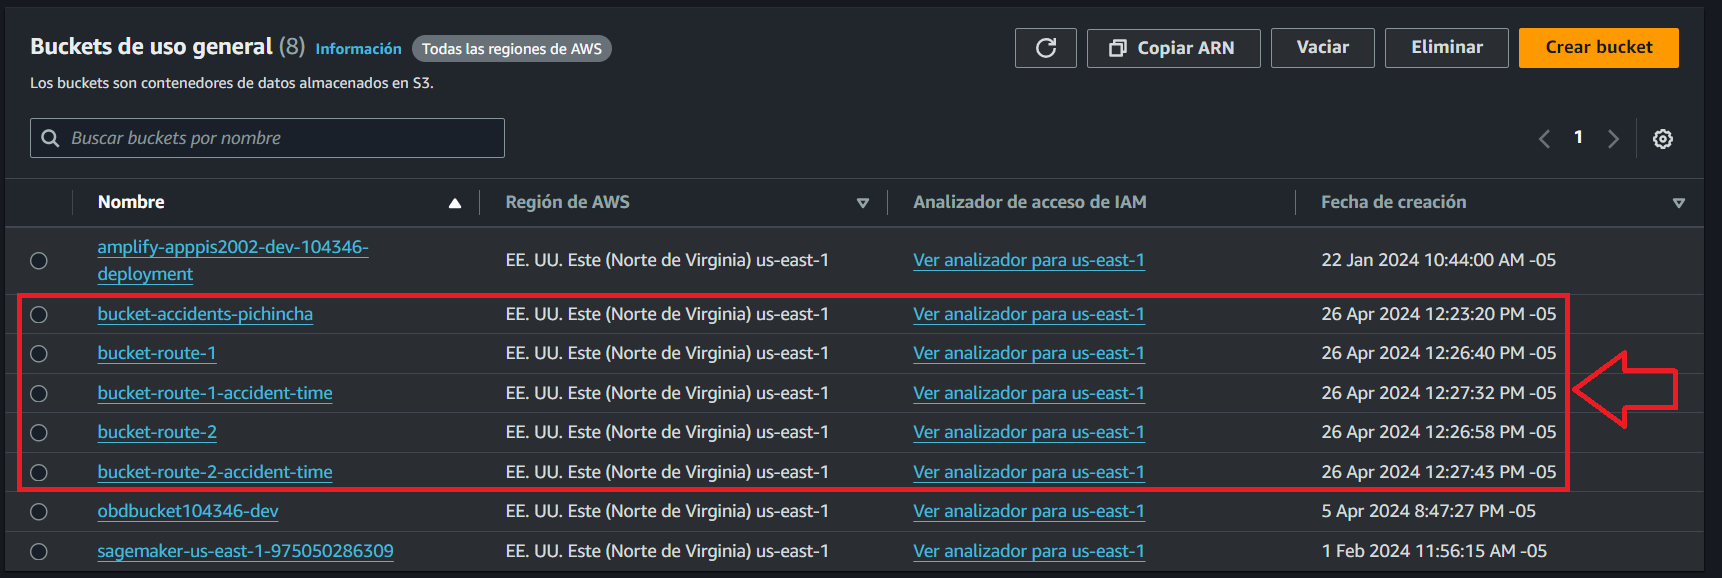
\includegraphics[width = 1\linewidth, height = 5.7cm]{Todos_Nuevo_Bucket_S3.png}
		\caption{Todos los Nuevos Buckets S3.}
		\label{Todos_Nuevo_Bucket_S3}
	\end{figure}
	\begin{figure}[!h]
		\centering
		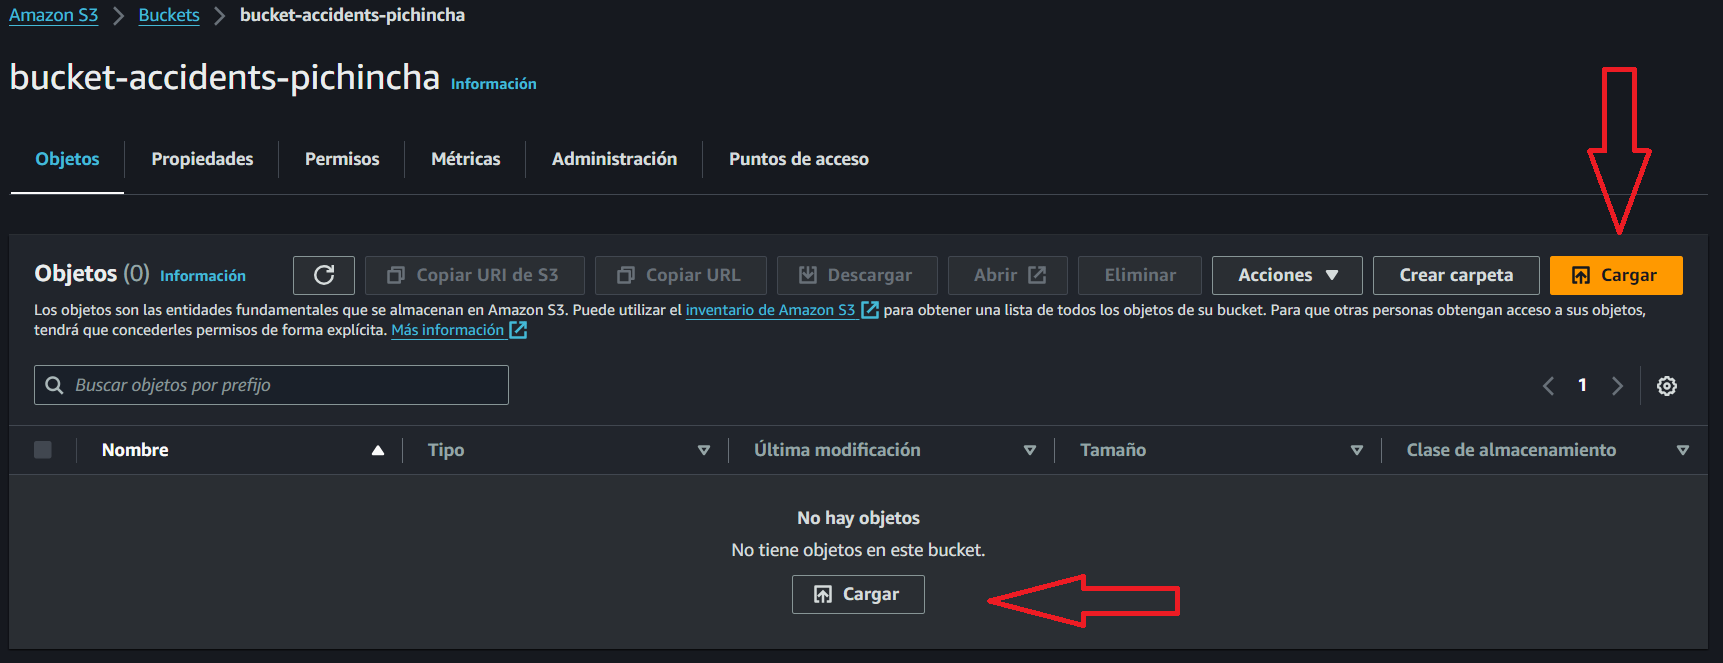
\includegraphics[width = 1\linewidth, height = 5.7cm]{Carga_Archivo_CSV_Nuevo_Bucket.png}
		\caption{Carga de Archivo CSV en el Bucket.}
		\label{Carga_Archivo_CSV_Nuevo_Bucket}
	\end{figure}
	\begin{figure}[!h]
		\centering
		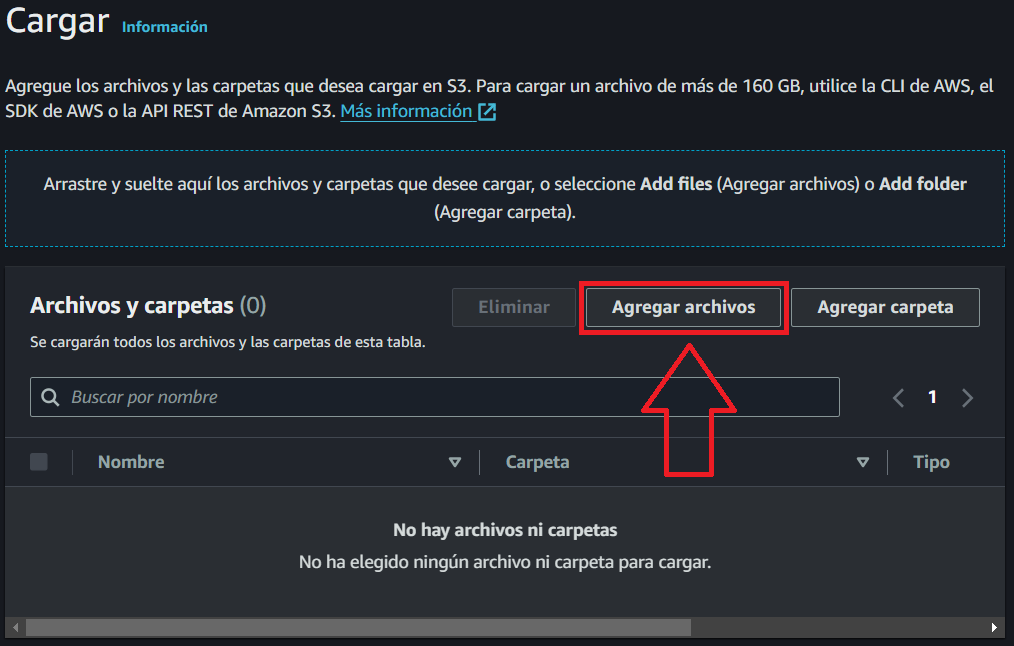
\includegraphics[width = 1\linewidth, height = 5.7cm]{Busqueda_Archivo_CSV_Bucket.png}
		\caption{Búsqueda de Archivo CSV del Bucket.}
		\label{Busqueda_Archivo_CSV_Bucket}
	\end{figure}
	\begin{figure}[!h]
		\centering
		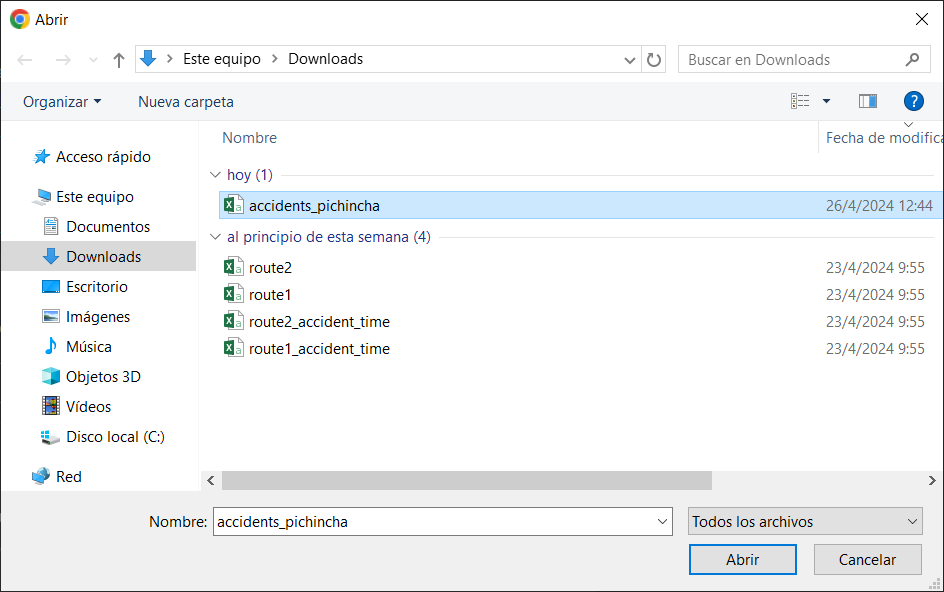
\includegraphics[width = 1\linewidth, height = 5cm]{Seleccion_Archivo_CSV_Bucket.png}
		\caption{Selección de Archivo CSV del Bucket.}
		\label{Seleccion_Archivo_CSV_Bucket}
	\end{figure}
	\begin{figure}[!h]
		\centering
		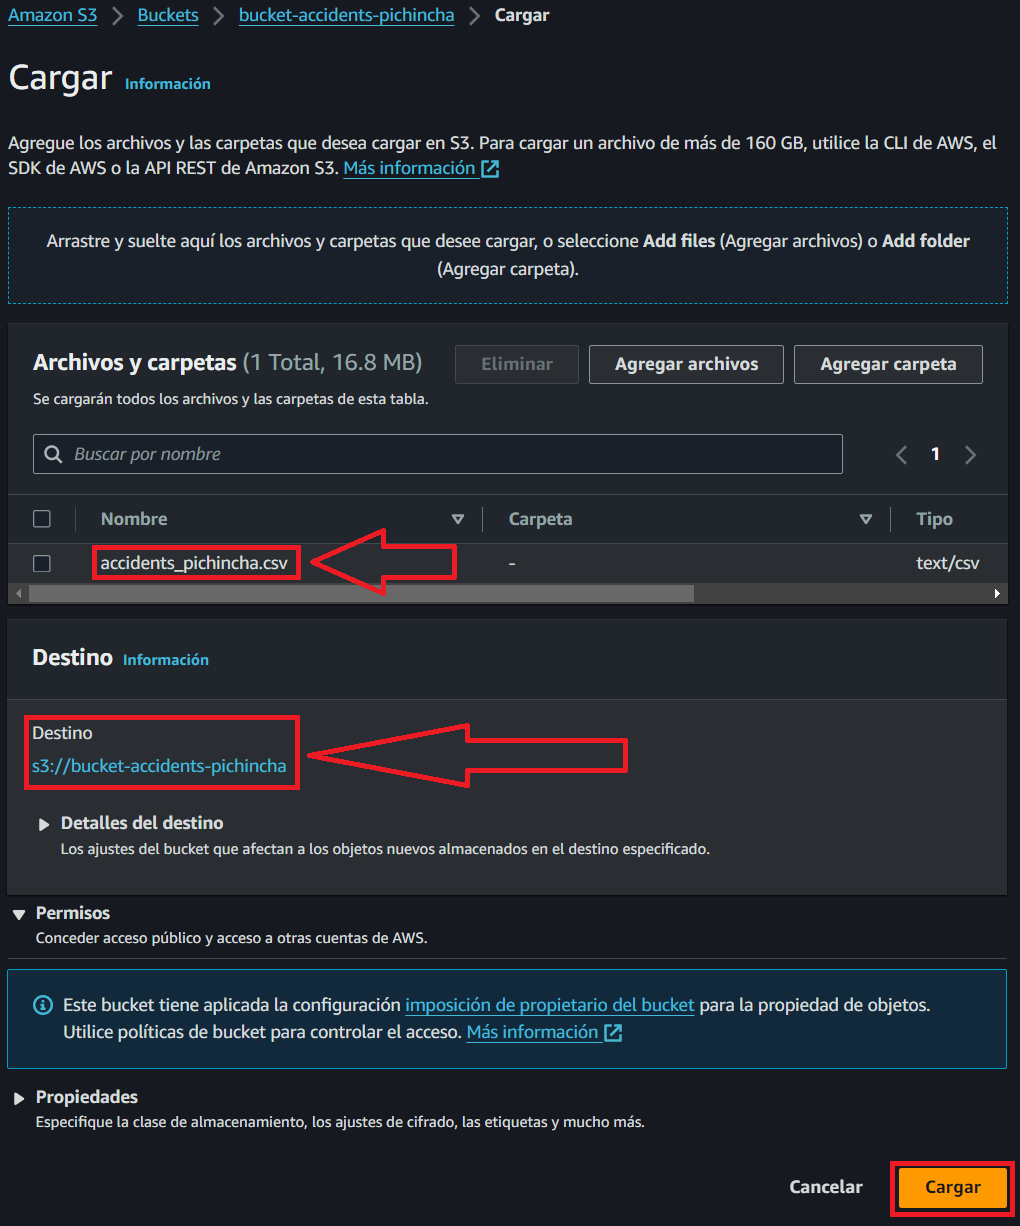
\includegraphics[width = 1\linewidth, height = 7.1cm]{Archivo_Destino_Bucket_S3.png}
		\caption{Configuración al Cargar Archivo al Bucket.}
		\label{Archivo_Destino_Bucket_S3}
	\end{figure}
	\begin{figure}[!h]
		\centering
		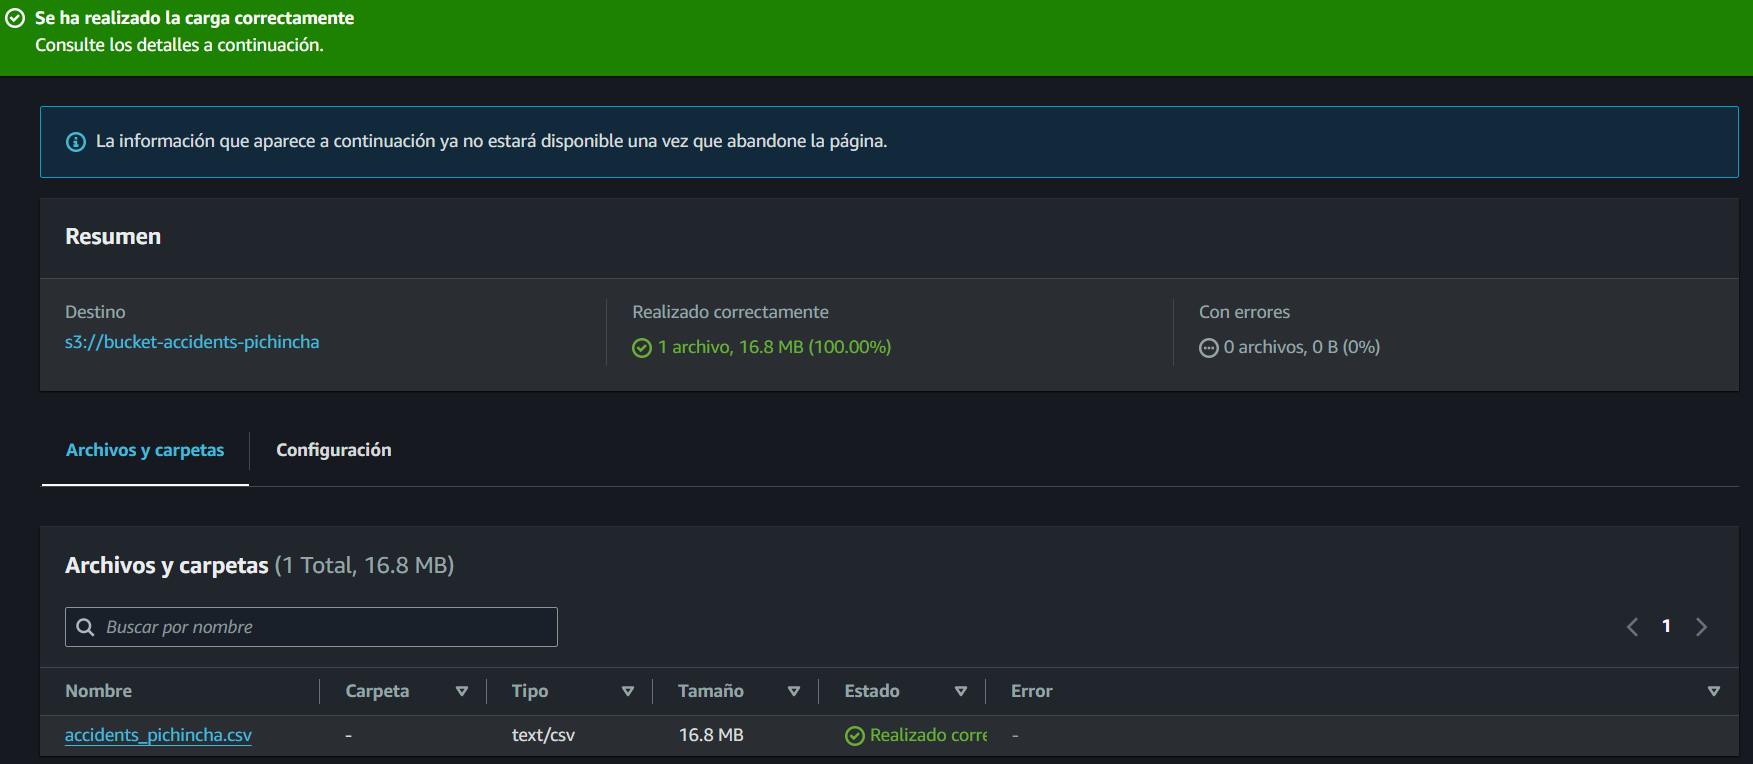
\includegraphics[width = 1\linewidth, height = 5cm]{Carga_Completa_Archivo_Bucket.png}
		\caption{Cargar Completa del Archivo al Bucket.}
		\label{Carga_Completa_Archivo_Bucket}
	\end{figure} \\
	\indent Recordar que este procedimiento de carga de archivos, es el mismo para todos los bucket creados con sus respectivos archivos CSV. Las Base de Datos utilizadas para ser subidas al bucket se encuentra en el siguiente enlace:
	\begin{itemize}
		\item \textcolor{blue}{\url{https://github.com/laboratorioAI/PIS_20_02_AGENTES_IA/tree/main/Actualizacion_2024/DataBases}}
	\end{itemize}
	\indent Una vez cargados los archivos CSV a sus respectivos bucket, el siguiente paso es ir a la consola de DynamoDB y escoger la opción de ``Importaciones de S3'' como muestra la Figura \ref{Importaciones_S3_Bucket}.
	\begin{figure}[!h]
		\centering
		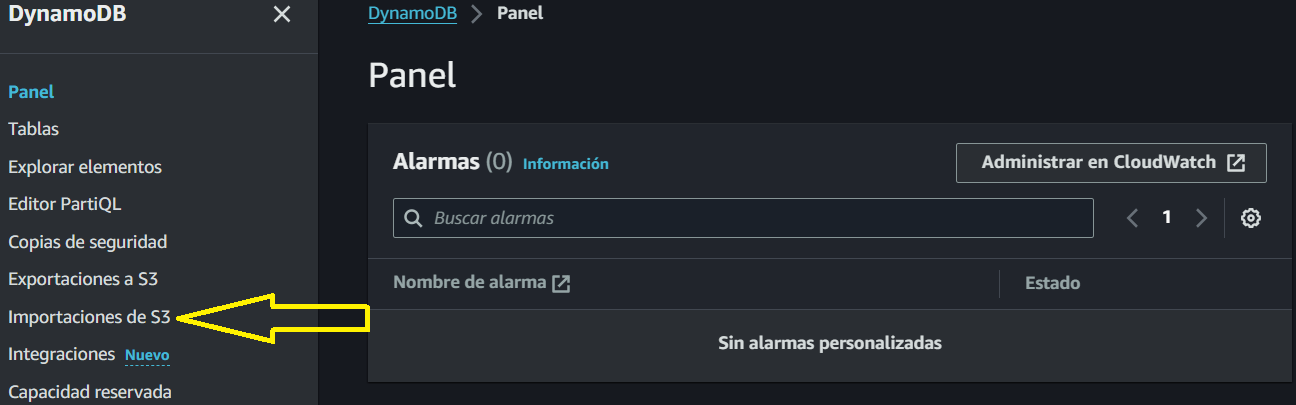
\includegraphics[width = 1\linewidth, height = 3.5cm]{Importaciones_S3_Bucket.png}
		\caption{Importaciones de S3.}
		\label{Importaciones_S3_Bucket}
	\end{figure} \\
	\indent Al presionar sobre ``Importaciones de S3'' se abrirá una nueva pantalla donde se deber presionar el botón ``Importaciones de S3'' como muestra la Figura \ref{Importaciones_S3_Bucket_2}
	\begin{figure}[!h]
		\centering
		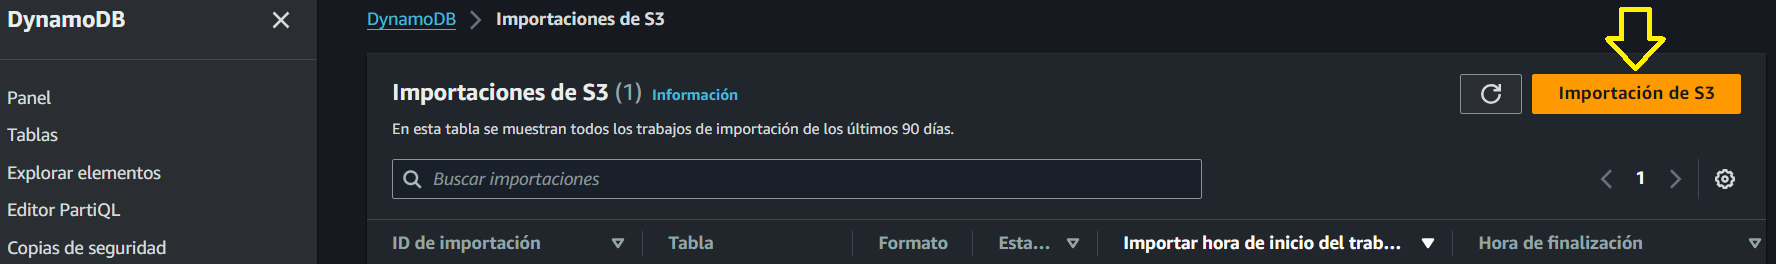
\includegraphics[width = 1\linewidth, height = 3.5cm]{Importaciones_S3_Bucket_2.png}
		\caption{Importaciones de S3 Parte 2.}
		\label{Importaciones_S3_Bucket_2}
	\end{figure} \\
	\indent En la nueva pantalla, se debe ir al apartado de ``URL de S3 fuente'' donde se debe ingresar la dirección ``Destino que se menciono anteriormente al cargar el archivo en el bucket. Ver Figura \ref{URL_S3_Fuente}.
	\begin{figure}[!h]
		\centering
		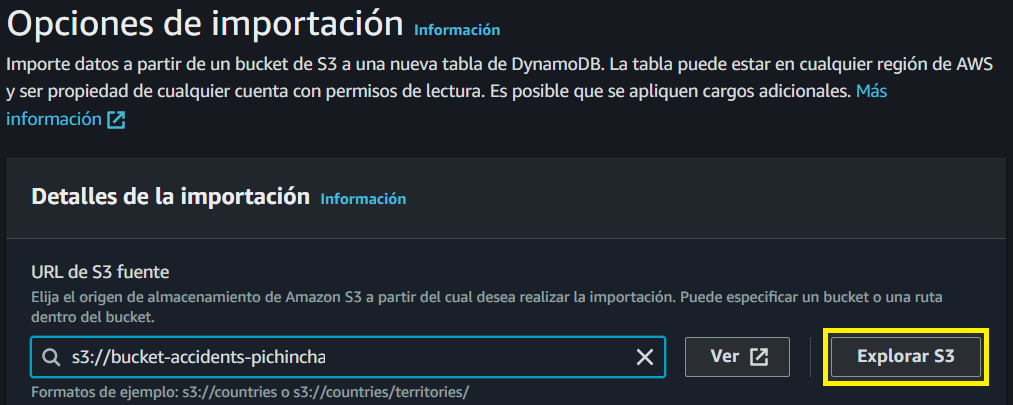
\includegraphics[width = 1\linewidth, height = 3.5cm]{URL_S3_Fuente.png}
		\caption{URL de S3 Fuente.}
		\label{URL_S3_Fuente}
	\end{figure} \\
	\indent Si no se recuerda la dirección ``Destino'' se puede presionar en ``Explorar S3'' (Ver Figura \ref{URL_S3_Fuente}) y allí desplegara todos los bucket y se escogerá con el cual se va a trabar y presionar el botón ``Elegir''. Ver Figura \ref{Explorador_Importaciones_S3}.
	\begin{figure}[!h]
		\centering
		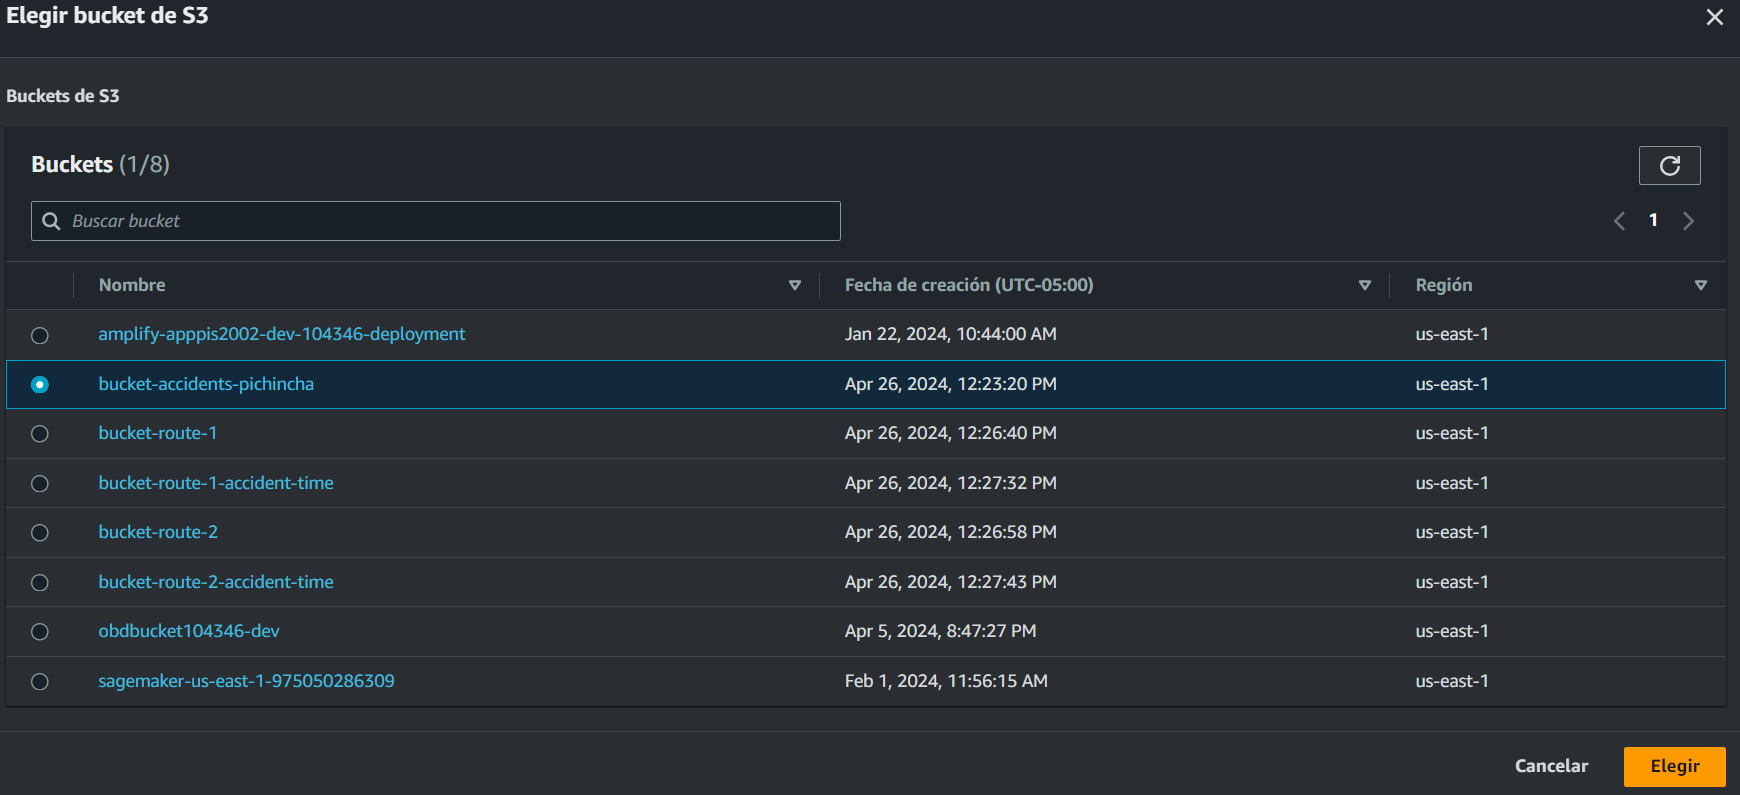
\includegraphics[width = 1\linewidth, height = 5cm]{Explorador_Importaciones_S3.png}
		\caption{Explorador S3.}
		\label{Explorador_Importaciones_S3}
	\end{figure} \\
	\indent Una vez que se escogió el bucket a trabajar se regresa a ``Opciones de importación'' y se complementa la configuración como se muestra en la Figura \ref{Detalles_Importaciones_S3}
	\begin{figure}[!h]
		\centering
		\includegraphics[width = 1\linewidth, height = 9.2cm]{Detalles_Importaciones_S3.png}
		\caption{Detalles Importación S3.}
		\label{Detalles_Importaciones_S3}
	\end{figure} \\
	\indent Configurado los detalles de la importación se presiona sobre el botón ``Siguiente'', esto llevara a ``Especificar los detalles de la tabla'' donde se  especificara detalles de la tabla como: Nombre de tabla, Clave de partición y Clave de ordenamiento, etc., como se muestra en la Figura \ref{Detalles_Tabla_Bucket}.
	\begin{figure}[!h]
		\centering
		\includegraphics[width = 1\linewidth, height = 5cm]{Detalles_Tabla_Bucket.png}
		\caption{Detalles Tabla DynamoDB.}
		\label{Detalles_Tabla_Bucket}
	\end{figure} \\
	\indent Terminado con ``Especificar los detalles de la tabla'' se continua con ``Configurar la configuración de la tabla - opcional'' don se especifica una serie de detalles opcionales como: Clases, Aprovisionamiento, Capacidad, etc. Ver Figura \ref{Configuracion_Opcional_Tabla_Bucket}.
	\begin{figure}[!h]
		\centering
		\includegraphics[width = 1\linewidth, height = 12cm]{Configuracion_Opcional_Tabla_Bucket.png}
		\caption{Configurar la configuración de la tabla - opcional.}
		\label{Configuracion_Opcional_Tabla_Bucket}
	\end{figure} \\
	\indent Posteriormente, se revisa en una vista detalla todas las configuraciones realizadas para verificar la correcta configuración, ver Figura \ref{Resumen_Detalle_Configuracion_Bucket}. 
	\begin{figure}[!h]
		\centering
		\includegraphics[width = 1\linewidth, height = 18.9cm]{Resumen_Detalle_Configuracion_Bucket.png}
		\caption{Resumen de la Configuración Realizada.}
		\label{Resumen_Detalle_Configuracion_Bucket}
	\end{figure} \\
	\indent Finalmente, se presiona el botón de ``Importar'' lo cual iniciara el proceso de importación, como muestra la Figura \ref{Iniciando_Importacion_Bucket_Tabla}.
	\begin{figure}[!h]
		\centering
		\includegraphics[width = 1\linewidth, height = 4.2cm]{Iniciando_Importacion_Bucket_Tabla.png}
		\caption{Iniciando Importación de Bucket a Tabla.}
		\label{Iniciando_Importacion_Bucket_Tabla}
	\end{figure} \\
	\indent Una vez que se haya terminado el proceso de importación se puede observar un mensaje de alerta informando que el proceso ha terminado correctamente como se puede ver en la Figura \ref{Proceso_Importacion_Finalizado_Bucket_Tabla}.
	\begin{figure}[!h]
		\centering
		\includegraphics[width = 1\linewidth, height = 4.2cm]{Proceso_Importacion_Finalizado_Bucket_Tabla.png}
		\caption{Proceso de Importación Finalizado de Bucket a Tabla.}
		\label{Proceso_Importacion_Finalizado_Bucket_Tabla}
	\end{figure} \\
	\indent Adicionalmente, en las tablas de DynamoDB se puede observar que se ha creado la tabla respectiva con el nombre y propiedades configuradas como muestra la Figura \ref{Tabla_Creada_Bucket_S3} y también, se puede ver que se ha creado el contenido dentro de la tabla como muestra la Figura \ref{Contenido_Tabla_Creada_Bucket_S3}.
	\begin{figure}[!h]
		\centering
		\includegraphics[width = 1\linewidth, height = 4.2cm]{Tabla_Creada_Bucket_S3.png}
		\caption{Tabla Creada en DynamoDB desde Bucket S3.}
		\label{Tabla_Creada_Bucket_S3}
	\end{figure}
	\begin{figure}[!h]
		\centering
		\includegraphics[width = 1\linewidth, height = 5cm]{Contenido_Tabla_Creada_Bucket_S3.png}
		\caption{Contenido de la Tabla Creada desde Bucket S3.}
		\label{Contenido_Tabla_Creada_Bucket_S3}
	\end{figure} \\
	\indent El procedimiento realizado en los pasos anteriores, se realiza para todas las tablas que se desee subir a DynamoDB. En la Figura \ref{Total_Importaciones_Bucket_S3} se muestra todas las importaciones realizadas y en la Figura \ref{Total_Tablas_Creadas_Bucket_S3} se muestra todas las tablas creadas en DynamoDB desde las importaciones de S3.
	\begin{figure}[!h]
		\centering
		\includegraphics[width = 1\linewidth, height = 5cm]{Total_Importaciones_Bucket_S3.png}
		\caption{Total de Importaciones de Bucket S3.}
		\label{Total_Importaciones_Bucket_S3}
	\end{figure}
	\begin{figure}[!h]
		\centering
		\includegraphics[width = 1\linewidth, height = 5cm]{Total_Tablas_Creadas_Bucket_S3.png}
		\caption{Total de Tablas Creadas desde Bucket S3.}
		\label{Total_Tablas_Creadas_Bucket_S3}
	\end{figure}  
	
	\section{Accuweather}\label{Etiqueta_Accuweather_Inc}
	AccuWeather Inc. es una empresa de medios estadounidense del sector privado que ofrece servicios comerciales de previsión meteorológica en todo el mundo. \\\newline
	\indent AccuWeather ofrece pronósticos y advertencias meteorológicas, así como productos y servicios meteorológicos adicionales, con clientes de todo el mundo en los medios de comunicación, las empresas y el gobierno, incluidas más de la mitad de las empresas Fortune 500 y miles de otras empresas en todo el mundo. También gestiona el sitio web gratuito ``AccuWeather.com'', un proveedor meteorológico en línea \cite{AccuWeather_2}.
	
	\subsection{Implementación de Servicios Accuweather}\label{Etiqueta_Servicios_Accuweather}
	Para iniciar con el uso de ``AccuWeather'' es necesario crear una cuenta en la pagina oficial de AccuWeather. En el siguiente enlace se puede registrar un nuevo usuario, en la sección ``Register'':
	\begin{itemize}
		\item \textcolor{blue}{\url{https://developer.accuweather.com/}}
	\end{itemize}
	\indent\newline\indent En esta sección el usuario deberá registrar us datos personales y aceptar las condiciones de servicio como muestra la Figura \ref{Registro_Nuevo_Usuario_AccuWeather}.
	\begin{figure}[!h]
		\centering
		\includegraphics[width = 1\linewidth, height = 10.5cm]{Registro_Nuevo_Usuario_AccuWeather.png}
		\caption{Registro de Nuevo Usuario en AccuWeather.}
		\label{Registro_Nuevo_Usuario_AccuWeather}
	\end{figure} \\
	\indent Una vez registrado se debe proceder con la ``Confirmación'' del registro en el correo proporcionado al momento de registrarse. Al correo proporcionado llegara un enlace que permitirá establecer la contraseña y realizar otras configuración como seleccionar la zona horaria. Ver Figura \ref{Confirmacion_Registro_Nuevo_Usuario_AccuWeather}.
	\begin{figure}[!h]
		\centering
		\includegraphics[width = 1\linewidth, height = 11cm]{Confirmacion_Registro_Nuevo_Usuario_AccuWeather.png}
		\caption{Confirmación Registro de Nuevo Usuario en AccuWeather.}
		\label{Confirmacion_Registro_Nuevo_Usuario_AccuWeather}
	\end{figure} \\
	\indent Finalizado con la confirmación de registro, se puede empezar a usar el sistema de AccuWeather. El primer paso es crear una nueva ``APP'' en la página principal como muestra la Figura \ref{Nueva_App_AccuWeather}.
	\begin{figure}[!h]
		\centering
		\includegraphics[width = 1\linewidth, height = 4.2cm]{Nueva_App_AccuWeather.png}
		\caption{Nueva App en AccuWeather.}
		\label{Nueva_App_AccuWeather}
	\end{figure} \\
	\indent Al crear la nueva App, se debe configurar una serie de parámetros como: Nombre, Tipo de API, Lenguaje de Programación, Alcance, etc. La Figura \ref{Configuracion_Nueva_APP_AccuWeather} muestra las configuraciones realizada a la nueva App en AccuWeather.
	\begin{figure}[!h]
		\centering
		\includegraphics[width = 1\linewidth, height = 11.7cm]{Configuracion_Nueva_APP_AccuWeather.png}
		\caption{Configuración  en Nueva APP de AccuWeather.}
		\label{Configuracion_Nueva_APP_AccuWeather}
	\end{figure} \\
	\indent Tras presionar el botón ``CREATE APP'' se regresara a la pantalla principal donde ya se podrá apreciar que la App ha sido creada exitosamente, ver Figura \ref{Nueva_APP_AccuWeather_Exito}.
	\begin{figure}[!h]
		\centering
		\includegraphics[width = 1\linewidth, height = 4cm]{Nueva_APP_AccuWeather_Exito.png}
		\caption{App creada en AccuWeather.}
		\label{Nueva_APP_AccuWeather_Exito}
	\end{figure} \\
	\indent Al ingresar a la App creada, en la sección ``Keys'' se puede encontrar la ``API Key'', que sera la llave con la cual se va a trabar en futuro. La Figura \ref{Api_Key_AccuWeather} muestra la llave creada.
	\begin{figure}[!h]
		\centering
		\includegraphics[width = 1\linewidth, height = 4.2cm]{Api_Key_AccuWeather.png}
		\caption{API Key de AccuWeather App.}
		\label{Api_Key_AccuWeather}
	\end{figure} \\
	\indent El siguiente paso es configurar la ``Locations API'' en la sección de ``API Reference'' como muestra la Figura \ref{Locations_API_AccuWeather}.
	\begin{figure}[!h]
		\centering
		\includegraphics[width = 1\linewidth, height = 4.2cm]{Locations_API_AccuWeather.png}
		\caption{Locations API de AccuWeather.}
		\label{Locations_API_AccuWeather}
	\end{figure} \\
	\indent Dentro de la opción ``Locations API'' Se debe buscar la opción ``Geoposition'' y escoger el método ``Geoposition Search'' el cual devuelve información sobre una ubicación específica, por Geo-Posición (Latitud y Longitud). Ver Figura \ref{AccuWeather_Geoposition_Option}.
	\begin{figure}[!h]
		\centering
		\includegraphics[width = 1\linewidth, height = 4.2cm]{AccuWeather_Geoposition_Option.png}
		\caption{AccuWeather Opción de Geo-Posicionamiento.}
		\label{AccuWeather_Geoposition_Option}
	\end{figure} \\
	\indent Al ingresar a la opción de búsqueda por Geo-Posicionamiento se ingresara a un  nuevo panel donde se debe configurar la opciones de búsqueda como: lenguaje, la clave, etc. Ver Figura \ref{AccuWeather_Geoposition_Configuracion}.
	\begin{figure}[!h]
		\centering
		\includegraphics[width = 1\linewidth, height = 3cm]{AccuWeather_Geoposition_Configuracion.png}
		\caption{Configuración de Geo-Posicionamiento.}
		\label{AccuWeather_Geoposition_Configuracion}
	\end{figure} \\
	\indent Una vez configurado, se presiona sobre el botón ``Send this request'' lo que realizara la petición y devolverá un resultado si la configuración fue realizada correctamente. De los resultados devueltos lo más importante, en este punto, es la ``Key'', ver Figura \ref{Resultados_Query_Geo_AccuWeather}. La Key es un valor que se utilizara para realizar la consulta de las condiciones climáticas.
	\begin{figure}[!h]
		\centering
		\includegraphics[width = 1\linewidth, height = 10.4cm]{Resultados_Query_Geo_AccuWeather.png}
		\caption{Resultados Consulta Geo-Posicionamiento.}
		\label{Resultados_Query_Geo_AccuWeather}
	\end{figure} \\
	\indent Con la Key se puede proceder con el siguiente paso. El siguiente paso consiste en crear la ``Current Conditions API'' que se encuentra en la sección de ``API Reference'' como muestra la Figura \ref{Current_Conditions_API_AccuWeather}.
	\begin{figure}[!h]
		\centering
		\includegraphics[width = 1\linewidth, height = 3cm]{Current_Conditions_API_AccuWeather.png}
		\caption{AccuWeather Opción de Current Conditions.}
		\label{Current_Conditions_API_AccuWeather}
	\end{figure} \\
	\indent Al igual que en el Geo-Posicionamiento, las ``Current Conditions'' requieren una configuración. En esta configuración se requiere la ``API Key''  y la ``Key'' generadas anteriormente. La Figura \ref{AccuWeather_Current_Conditions_Configuracion} muestra la configuración realizada.
	\begin{figure}[!h]
		\centering
		\includegraphics[width = 1\linewidth, height = 3cm]{AccuWeather_Current_Conditions_Configuracion.png}
		\caption{Configuración de Condiciones Actuales.}
		\label{AccuWeather_Current_Conditions_Configuracion}
	\end{figure} \\
	\indent Una vez configurado, se presiona sobre el botón ``Send this request'' lo que realizara la petición y devolverá un resultado si la configuración fue realizada correctamente. En los resultados devuelto se puede observar las condiciones climáticas actuales para el punto dado mediante geo-posicionamiento, ver Figura \ref{Resultados_Query_Current_AccuWeather}.
	\begin{figure}[!h]
		\centering
		\includegraphics[width = 0.65\linewidth, height = 7.4cm]{Resultados_Query_Current_AccuWeather.png}
		\caption{Resultados Consulta Condiciones Actuales.}
		\label{Resultados_Query_Current_AccuWeather}
	\end{figure} 
	
	\section{Resultados}\label{Resultados}
	Una vez completado el desarrollo, se genera un archivo APK (Archivo de Paquete de Android), que es el paquete final de la aplicación. Este archivo contiene todos los recursos necesarios para instalar y ejecutar la aplicación en dispositivos Android. La aplicación se puede distribuir a través de la tienda de aplicaciones de Google Play o mediante otros métodos de distribución, como la instalación directa desde un sitio web. \\\newline
	\indent Los resultados obtenidos tras la ejecución del proyecto son las siguientes:
	\begin{itemize}
		\item Aplicación móvil (agente de adquisición) para recolección y almacenamiento de información proveniente de un escáner OBD2, un receptor GPS, un reloj inteligente, un servicio web y de una base de datos.
		\item Conjunto de datos de conducción denominado POLIDriving.
		\item Herramienta basada en servicios de nube (agente de procesamiento) para lectura de datos de conducción, procesamiento de información a través de un modelo de aprendizaje y almacenamiento de resultados en una base de datos.
		\item Aplicación móvil (agente de respuesta) para consulta y presentación de niveles de riesgo de accidentes a usuarios finales (conductores).
		\item Esquema de seguridad basado en computación criptográfica para protección de información intercambiada entre agentes.
	\end{itemize}
	
	\section{Ayudas Técnicas}\label{Ayudas_Tecnicas}
	La siguiente lista de enlaces presentan ayudas a la implementación de los servicios vistos en este documento:
	\begin{itemize}
		\item \textcolor{blue}{\url{https://www.youtube.com/watch?v=JU_2uDnR-Yk}}
	\end{itemize}
		
	\bibliography{Bibliografia}
	\bibliographystyle{apalike}
\end{document}